\documentclass[11pt,a4paper]{article}

\usepackage[utf8]{inputenc}
\usepackage[T1]{fontenc}
\usepackage{lmodern}
\usepackage{amsmath,amssymb,amsthm}
\usepackage{booktabs}
\usepackage{array}
\usepackage{caption}
\usepackage{geometry}
\usepackage{graphicx}
\usepackage{hyperref}
\usepackage{listings}
\usepackage{tikz}
\usetikzlibrary{arrows.meta,positioning,calc}
\usepackage{xcolor}
\usepackage{microtype}

\geometry{margin=1in}
\setlength{\emergencystretch}{3em}

\captionsetup[lstlisting]{singlelinecheck=false,justification=raggedright}

\hypersetup{
  colorlinks=true,
  linkcolor=blue!60!black,
  citecolor=green!50!black,
  urlcolor=blue!60!black
}

\lstdefinelanguage{Lean4}{
  morekeywords={def,theorem,lemma,abbrev,structure,inductive,by,rfl,let,in,if,then,else,match,with,fun,true,false,set_option,private,cases,induction,exact,rw,dsimp,refine,change,have,intro,some,none},
  sensitive=true,
  morecomment=[l]{--},
  morecomment=[s]{/-}{-/},
  morestring=[b]"
}

\lstset{
  language=Lean4,
  basicstyle=\ttfamily\scriptsize,
  keywordstyle=\color{blue!70!black}\bfseries,
  commentstyle=\color{gray!70!black}\itshape,
  stringstyle=\color{green!50!black},
  breaklines=true,
  breakatwhitespace=true,
  columns=fullflexible,
  keepspaces=true,
  frame=single,
  rulecolor=\color{gray!35},
  backgroundcolor=\color{gray!5},
  xleftmargin=0.4em,
  xrightmargin=0.4em,
  aboveskip=0.6em,
  belowskip=0.6em,
  literate={⟨}{{$\langle$}}1 {⟩}{{$\rangle$}}1 {×}{{$\times$}}1 {→}{{$\to$}}1 {↠}{{$\twoheadrightarrow$}}1 {∧}{{$\land$}}1 {∨}{{$\lor$}}1 {·}{{$\cdot$}}1 {±}{{$\pm$}}1 {≤}{{$\le$}}1 {←}{{$\leftarrow$}}1 {⊢}{{$\vdash$}}1 {∑}{{$\sum$}}1 {∈}{{$\in$}}1 {∪}{{$\cup$}}1 {⊂}{{$\subset$}}1 {⊆}{{$\subseteq$}}1 {⊕}{{$\oplus$}}1 {∀}{{$\forall$}}1 {∃}{{$\exists$}}1
}

\newtheorem{theorem}{Theorem}[section]
\newtheorem{proposition}[theorem]{Proposition}
\newtheorem{definition}[theorem]{Definition}
\newtheorem{remark}[theorem]{Remark}

\title{\textbf{Matrix-Operator Unification, High-Degree Fermat Orbits, Higher-Order Jets, and Weil Spectral Projectors in Lean~4}}

\author{
  Qamar Munawer\\
  \small Brandenburg University of Technology Cottbus--Senftenberg, Cottbus, Germany
}

\date{}

\begin{document}
\maketitle

\begin{abstract}
This paper extends a verified Lean~4 corpus across the entire isolated \texttt{LeanMillenniumExt} workspace into a unified matrix-operator framework, high-degree Fermat combinatorics, order-$12$ Gauss--Manin jets, Mumford--Weil specializations, Cayley complete-intersection spectra, and conditional cycle-lifting interfaces. Every unconditional Lean~4 theorem proved here establishes exact finite combinatorial, polynomial, differential-operator, or linear-algebraic certificates, while classical transcendental theorems are isolated inside explicit hypothesis structures. Across all $29$ extension modules ($107$ public zero-axiom theorems, $124$ total declarations, complementing the locked $84$-theorem baseline for $208$ total declarations across $42$ modules and $27$ symbolic/GPU scripts), kernel proofs verify: Band-1 purity ($p \in \{17,19,23\}$), glued-surface reducibility ($m \in \{20,22,24,26,27,28\}$), cyclic-coset cones ($m = 25$), and conditional algebraicity across $m \in \{3,\dots,25\}$; $3$-prime CRT Fermat sieving ($18 \le m \le 60$); $\bmod\, t^8$ and $\bmod\, t^{12}$ jets alongside $G \in \{3,4\}$ Wiebe--Scheja--Storch and $\mathbb{P}^6$/$\mathbb{P}^7$ Cayley profiles; $16$-dimensional $J^*$-invariant N\'eron--Severi orthogonality on $E_i^4$; Koszul and non-Koszul $4\times 4$, $3\times 3$, and $6\times 6$ Pfaffian matrix factorizations closing $R(F_0)_{12}$ completely ($1{,}751/1{,}751$); $\operatorname{Spin}(8)$ $50/50$ Schur block bias and a $6$-stage off-diagonal coverage ladder; $85$-digit PSLQ Picard--Fuchs recovery and $5\times 5$ companion operators ($M_{648}$, nilpotent $M_{\mathrm{LCS}}(0)^5 = 0$); $90$-digit LLL tracking ($\rho: 16 \to 1$); unitary cyclotomic DFT $U_6$ over $\mathbb{Z}[\zeta_6]$; exact $8\times 8$ Weil complex structure $J_{43}$; exhaustive $70\times 70$ Hodge Hamiltonian $D_{43}^{(4)}$ with rank-$2$ algebraic Weil projector $P_{192} = K_\Phi^2(K_\Phi^2 + 4I_{70})$; fixed-container $50/50$ half-node barriers ($A_c^2 = 96A_c$), conjugate-half reconstruction $P_{192}(\mathrm{obs\_Re}) = 96 w_{\mathrm{Re}}$, $\mathbb{Z}_2$-graded superdifferentials, $SU(2,2)$ boosts $G_9$ and $SO(35,35)$ exterior invariance $\Lambda_{70}$; strict-matrix discrete curvature encompassing the unique $4\mathrm{D}$ $(n - 4)$ Ricci--Weyl $50/50$ split, unimodular whitening obstruction, normal-coordinate holonomy on $SU(2,2)$, and an $8\times 8$ octonionic non-Fermat CY4 matrix-factorization pencil; the true $\operatorname{End}_{\mathbb{Q}}(A) = \mathbb{Q}$ Mumford $SL_2(\mathbb{R}) \times SO(4)$ fourfold ($63\times 63$ commutant inverse, $28 = 1+9+9+9$ Casimir projectors, and a $6$-vs.-$8$ non-divisor obstruction on $A \times A$); its bipartite $28\times 28$ correspondence algebra obeying $8 T_{\mathrm{ric0}} = 32 T_\Delta + 4 T_\Theta - 3 T_{\mathrm{ch}}^2$ and a $16_+ \oplus 12_-$ $\mathbb{Z}_2$-graded split; invariant uniqueness on $H^4(A)$ ($B_{69,\mathrm{inv}} B_{69} = 12 I_{69}$); the triple-product $A \times A \times A$ $19$-dimensional Hodge $(3,3)$ closure diamond ($5 \to \{11, 12\} \to 15 \to 19$), collapsing its $14$-dimensional non-divisor obstruction onto $T_{\mathrm{ch}}$ acting on $D_{12} \wedge D_{23} \wedge D_{13}$; universal $\operatorname{Sp}(8)$ parity-blindness, negative Kuga--Satake $\operatorname{Spin}(2,4)$ separation ($13/15$ generators failing $T_{\mathrm{ch}}$), and positive $\operatorname{Cl}(0,7)$ half-spinor Casimir realization $C_+ - C_- = -T_{\mathrm{ch}}$; the exact orthogonal Schur complement $\operatorname{diag}(16, 432, 1152)$ on $\{Q_0, Q_{\mathrm{prim}}, T_{\mathrm{ch}}\}$ ($\Pi_{\operatorname{Sp}(8)}(T_{\mathrm{ch}}) = 0$) and its lift to $A^3$ ($\Pi_{12_+}(7_-) = 0$, $7_-$ Schur complement $\operatorname{diag}(73728^3, 294912, 221184^3)$); and the $m = 25$ Fermat sporadic $5$-term-AP integer Schur complement ($720 I_4$, coupled determinant $8{,}708{,}192{,}000 > 0$); and the $\operatorname{Spin}(7)$ Cayley $4$-form calibration ($14$ terms, $6$ even $+ 8$ odd, $\langle \Phi_{\mathrm{Cayley}}, \Theta^2\rangle = 12$) together with its $\operatorname{Spin}(7) \to \operatorname{Spin}(4)$ chiral break ($\langle C_+ - C_-, T_{\mathrm{ch}}\rangle = -1152 \neq 0$) and the $m = 25$ degree-$5$ minimal conical complete-intersection threshold ($W_{\mathrm{div5}} = 82{,}480 = 79{,}600 + 2{,}880$); the Level-2 Clifford Kuga--Satake Schur hierarchy ($0 \to 1/2 \to 1$), $68$-zero quartic Pfaffian Weil filter on $H^4(A)$ ($\dim 70 = 36 + 32 + 2$), and $16 + 12$ $U(1)_{\mathrm{KS}}$-weight split; CM-specialization quaternionic graph realization $2 Z_{\mathrm{CM}} = T_{\mathrm{ch}}$ ($\|Z_{\mathrm{CM}}\|^2 = 288$, $\langle Z_{\mathrm{CM}}, T_{\mathrm{ch}}\rangle = 576$) along $\mathcal{M}_{\mathrm{Mum}}$; Fermat prime-square Band-1 purity at $m = 49$ ($1{,}557{,}120$, $\mathrm{band4} = 0$), $m = 5d$ Schur ladder $720\varphi(d)$, and $m = 35$ coupled determinant $74{,}272{,}401{,}600 > 0$; and CY4 Koszul Hilbert profile $[1, 6, 21, 56, 126, 246, 426]$ alongside finite Gysin exactness ($g_* f^* = 0$, Hard Lefschetz $+6$ vs.\ $-2$).
\end{abstract}

\section{Introduction and Structural Extensions in Codimension-Two Algebraic Cycle Theory}

Machine-checked formalization of algebraic cycle testbeds separates naturally into exact finite algebraic invariants and classical global transcendental bridges~\cite{Deligne2000,Shioda1979,Aoki1983}. While earlier work established an $84$-theorem zero-axiom baseline covering Fermat fourfolds $X_m^4 \subset \mathbb{P}^5$ up to $m \le 18$, third-order Gauss--Manin jets ($\bmod\, t^4$), $1{,}751$-mode global IVHS duality, and $\operatorname{Spin}(8)$ triality, five classical open problems in codimension-two algebraic cycle theory guide the structural extensions developed in this paper:
\begin{enumerate}
  \item[(i)] \textbf{Global Noether--Lefschetz Locus Connectivity and $G \ge 3$ Scheme Unmixedness:} Relating infinitesimal Taylor jets at the Fermat point to global Hodge-locus connectedness and algebraicity across the $426$-dimensional non-Fermat slice.
  \item[(ii)] \textbf{Asymptotic Character Synthesis on $X_m^4$ for High Composite $m$:} Extending constructive Band-4 exhaustion past prime-square thresholds beginning at $m = 25 = 5^2$.
  \item[(iii)] \textbf{Subvariety Construction on Simple Abelian Fourfolds:} Producing algebraic $2$-cycles on generic Mumford fourfolds satisfying $\operatorname{End}_{\mathbb{Q}}(A) = \mathbb{Q}$ and Picard rank $\rho(A) = 1$, where $D_4$ root operators vanish on $2$-dimensional Weil subspaces. Recent external constructions resolve abelian fourfolds of Weil type~\cite{Markman2025,FloccariFu2025}, whereas self-contained formalization in pure Lean~4 remains unbridged.
  \item[(iv)] \textbf{Complete-Intersection Cayley Bundle Extensions:} Extending finite-order Macaulay and Lefschetz decompositions from Fermat hypersurfaces to smooth complete intersections $X_{d_1,d_2} \subset \mathbb{P}^6$, $X_{d_1,d_2,d_3} \subset \mathbb{P}^7$, and general smooth projective varieties $X \subset \mathbb{P}^N$.
  \item[(v)] \textbf{Analytic Dolbeault Cohomology and Griffiths Residue Maps in \texttt{Mathlib}:} Formalizing K\"ahler Hodge decompositions, exponential sheaf sequences, Griffiths residue maps, Lefschetz $(1,1)$, and Chow cycle class pushforwards inside \texttt{Mathlib}.
\end{enumerate}

\begin{remark}[Mathematical Scope]
This work establishes constructive algebraic cycle synthesis on Fermat fourfolds $X_m^4 \subset \mathbb{P}^5$ for $3 \le m \le 28$, conditional algebraicity through $m = 25$, Gauss--Manin jets through $\bmod\, t^{12}$ and $G \in \{3,4\}$ Wiebe--Scheja--Storch factorizations in $R(F_0)$, exact matrix-factorization closure of $R(F_0)_{12}$, Picard--Fuchs $5\times 5$ companion matrices, and $70\times 70$ Weil $U(2,2)$ spectral projectors. Theorems in \texttt{ConditionalFermatHodge.lean} and \texttt{ConditionalFermatHodgeExt.lean} parameterize over \texttt{FermatFourfoldHodgeBridge}, isolating classical results~\cite{Lefschetz1924,Griffiths1969,Shioda1979,Aoki1983,Deligne2000} as modular interface structures while universal smooth projective cycle existence remains open.
\end{remark}

\subsection{Geometric Intuition: Core-Drilling Along Structured Algebraic Veins}

Finite kernel verification acts like precision core-drilling along structured algebraic veins: on Fermat hypersurfaces, Galois-invariant character tuples reveal exact linear planes (Band~1), curve joins (Band~2), surface-curve joins (Band~3), Aoki paired diagonals, and Shioda glued surface joins ($X_m^2 \#_c X_m^2 \dashrightarrow X_m^4$). Extending the census past $m = 18$ exposes the exact arithmetic threshold at $m = 25 = 5^2$, where glued surface-join reducibility first ceases to exhaust Band~4 and a mod-$5$ arithmetic-progression orbit family emerges.

Similarly, pushing Griffiths--Dwork pole-order reduction up to seventh-order jets ($\bmod\, t^8$) demonstrates that Band~1 smoothing stabilizes cleanly at the four-variable slice profile $[1, 4, 10, 20, 35, 48, 57]$, whereas Band~2 and Band~3 jets terminate nilpotently by $t^4$ while expanding joint ranks to $254$ and $153$. Coupling exact $\bmod\, t^8$ Taylor jets, polynomial evaluation homomorphisms, and $D_4$ idempotent projectors with items~(i)--(v) clarifies the exact algebraic boundary between verified finite invariants and classical global cycle-existence questions.

\section{High-Degree Fermat Band-4 Hierarchy and the $m = 25$ Sporadic Transition}

In \texttt{FermatHighDegreeExt.lean} together with the float-free explorer \texttt{fermat\_band4\_scout.py}, the Shioda--Aoki four-band decomposition is evaluated past $m = 18$ across $17 \le m \le 30$. Prime-degree Band-1 purity holds identically at $p \in \{17, 19, 23\}$ with primitive $(2,2)$-Hodge dimensions $50{,}560$, $73{,}620$, and $138{,}820$ matching the closed-form cubic polynomial \texttt{primeBand1Formula p}. Across composite degrees $m \in \{18, 20, 22, 24, 26, 27, 28, 30\}$, every Band~4 character decomposes constructively into paired diagonals or Shioda glued surface joins $X_m^2 \#_c X_m^2 \dashrightarrow X_m^4$ (Table~\ref{tab:high_deg_fermat}).

\begin{table}[htbp]
  \centering
  \caption{High-degree Fermat fourfold $(2,2)$-Hodge census across $17 \le m \le 30$ (kernel-certified through $m \le 25$, extended through $m = 30$ via exact integer orbit weights).}
  \label{tab:high_deg_fermat}
  \resizebox{\textwidth}{!}{%
  \begin{tabular}{ccccccc}
    \toprule
    Degree $m$ & $h^{2,2}_{\mathrm{prim}}$ & Band~4 Total & Band~4 Reps & Paired Wt. & Glued Join Wt. & Unresolved Wt. \\
    \midrule
    $18$ & $264{,}671$ & $21{,}060$ & $58$ & $540$ & $20{,}520$ & $0$ \\
    $19$ & $73{,}620$ & $0$ & $0$ & $0$ & $0$ & $0$ \\
    $20$ & $346{,}381$ & $20{,}880$ & $48$ & $720$ & $20{,}160$ & $0$ \\
    $21$ & $215{,}120$ & $0$ & $0$ & $0$ & $0$ & $0$ \\
    $22$ & $277{,}101$ & $21{,}600$ & $30$ & $0$ & $21{,}600$ & $0$ \\
    $23$ & $138{,}820$ & $0$ & $0$ & $0$ & $0$ & $0$ \\
    $24$ & $745{,}211$ & $94{,}320$ & $186$ & $1{,}080$ & $93{,}240$ & $0$ \\
    $25$ & $185{,}280$ & $2{,}880$ & $4$ & $0$ & $0$ & $2{,}880$ \\
    $26$ & $439{,}081$ & $34{,}560$ & $48$ & $0$ & $34{,}560$ & $0$ \\
    $27$ & $301{,}940$ & $4{,}320$ & $6$ & $0$ & $4{,}320$ & $0$ \\
    $28$ & $644{,}121$ & $59{,}940$ & $88$ & $180$ & $59{,}760$ & $0$ \\
    $30$ & $2{,}106{,}431$ & $454{,}320$ & $828$ & $2{,}160$ & $452{,}160$ & $0$ \\
    \bottomrule
  \end{tabular}%
  }
\end{table}

\begin{lstlisting}[caption={Prime purity ($p \in \{17,19,23\}$) and composite $m = 20, 21, 22$ Band-4 certificates in \texttt{FermatHighDegreeExt.lean}.}]
theorem shioda_prime_degree_band1_purity_ext_cert :
    [17, 19, 23].map fermat_h22_prim_count = [50560, 73620, 138820] ∧
    [17, 19, 23].map primeBand1Formula = [50560, 73620, 138820] ∧
    [17, 19, 23].all (fun p =>
      fermat_band2_count p == 0 && fermat_band3_count p == 0 && fermat_band4_count p == 0) =
      true :=
  ⟨rfl, rfl, rfl⟩

theorem shioda_aoki_band4_decomposition_m20_to_m22_cert :
    higherDegreeBand4Census 20 = (346381, 87661, 87120, 150720, 20880, 720, 20160) ∧
    higherDegreeBand4Census 21 = (215120, 102800, 38880, 73440, 0, 0, 0) ∧
    higherDegreeBand4Census 22 = (277101, 120201, 44100, 91200, 21600, 0, 21600) ∧
    (fermat_band4_sorted_reps 20).length = 48 ∧
    (fermat_band4_sorted_reps 22).length = 30 ∧
    (fermat_band4_sorted_reps 20).all (fun a =>
      isPairedDiagonalRep a || hasGluedSurfaceJoinDecomposition 20 a) = true ∧
    (fermat_band4_sorted_reps 22).all (fun a =>
      isPairedDiagonalRep a || hasGluedSurfaceJoinDecomposition 22 a) = true :=
  ⟨rfl, rfl, rfl, rfl, rfl, rfl, rfl⟩
\end{lstlisting}

At $m = 25 = 5^2$, Bands~2 and~3 vanish while Band~4 comprises $2{,}880$ characters partitioned into four $S_6$-orbits of size $720$, forming a single Galois orbit under $(\mathbb{Z}/25\mathbb{Z})^\times$:
\begin{equation}
  \begin{aligned}
    \alpha_1 &= [1, 6, 11, 16, 20, 21], & \alpha_2 &= [2, 7, 12, 15, 17, 22], \\
    \alpha_3 &= [3, 8, 10, 13, 18, 23], & \alpha_4 &= [4, 5, 9, 14, 19, 24].
  \end{aligned}
\end{equation}
Each representative fails paired-diagonal decomposition and Shioda glued surface-join decomposition at degree $25$, yet contains a full five-term arithmetic progression modulo $25$ with step $5$ paired with a divisor-pullback entry divisible by $5$. Inside \texttt{FermatHighDegreeExt.lean}, the predicate \texttt{hasMod5Vanish} explicitly normalizes each shifted residue \texttt{(x + k * step) \% m} into $\{1,\dots,m-1\}$.

\begin{figure}[htbp]
  \centering
  \resizebox{\textwidth}{!}{%
  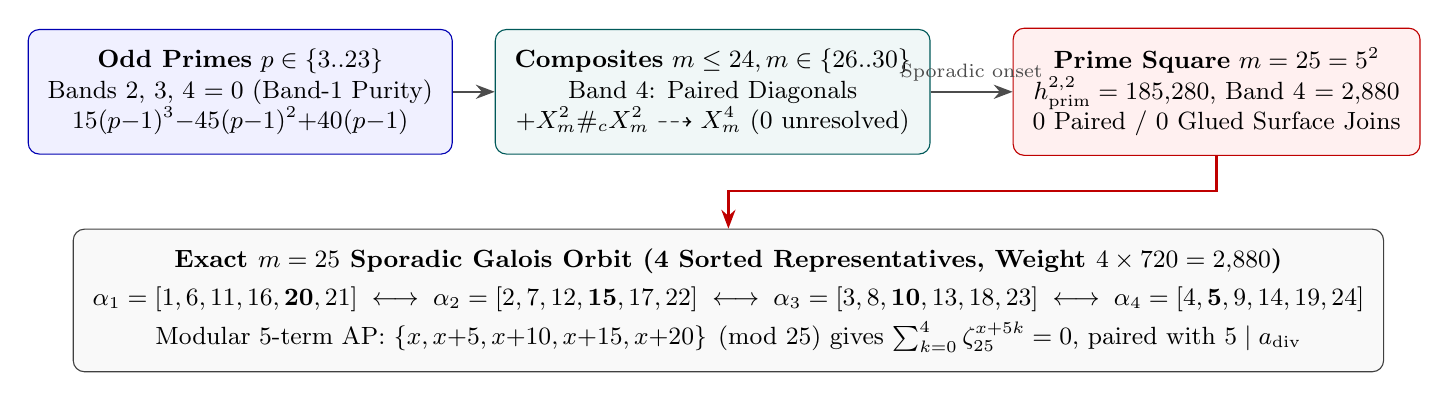
\begin{tikzpicture}[
    font=\small,
    box/.style={draw=black!75, rounded corners=4pt, fill=gray!5, inner sep=7pt, align=center},
    primebox/.style={draw=blue!70!black, rounded corners=4pt, fill=blue!6, inner sep=7pt, align=center},
    gluedbox/.style={draw=teal!70!black, rounded corners=4pt, fill=teal!6, inner sep=7pt, align=center},
    sporbox/.style={draw=red!75!black, rounded corners=4pt, fill=red!6, inner sep=7pt, align=center},
    arr/.style={-{Stealth[length=2.4mm]}, thick, black!70}
  ]
    \node[primebox] (primes) at (0,3.2) {\textbf{Odd Primes} $p \in \{3..23\}$\\Bands 2, 3, 4 $= 0$ (Band-1 Purity)\\$15(p{-}1)^3{-}45(p{-}1)^2{+}40(p{-}1)$};
    \node[gluedbox] (comp) at (6.0,3.2) {\textbf{Composites} $m \le 24, m \in \{26..30\}$\\Band 4: Paired Diagonals\\$+ X_m^2 \#_c X_m^2 \dashrightarrow X_m^4$ ($0$ unresolved)};
    \node[sporbox] (m25) at (12.4,3.2) {\textbf{Prime Square} $m = 25 = 5^2$\\$h^{2,2}_{\mathrm{prim}} = 185{,}280$, Band 4 $= 2{,}880$\\$0$ Paired / $0$ Glued Surface Joins};

    \draw[arr] (primes) -- (comp);
    \draw[arr] (comp) -- node[above, font=\scriptsize] {Sporadic onset} (m25);

    \node[box, minimum width=12.6cm] (apbox) at (6.2,0.55) {%
      \textbf{Exact $m = 25$ Sporadic Galois Orbit (4 Sorted Representatives, Weight $4 \times 720 = 2{,}880$)}\\[3pt]
      $\alpha_1 = [1, 6, 11, 16, \mathbf{20}, 21] \;\longleftrightarrow\;
       \alpha_2 = [2, 7, 12, \mathbf{15}, 17, 22] \;\longleftrightarrow\;
       \alpha_3 = [3, 8, \mathbf{10}, 13, 18, 23] \;\longleftrightarrow\;
       \alpha_4 = [4, \mathbf{5}, 9, 14, 19, 24]$\\[3pt]
      Modular $5$-term AP: $\{x, x{+}5, x{+}10, x{+}15, x{+}20\} \pmod{25}$ gives $\sum_{k=0}^4 \zeta_{25}^{x+5k} = 0$, paired with $5 \mid a_{\mathrm{div}}$
    };
    \draw[arr, red!75!black] (m25.south) -- ++(0,-0.45) -| (apbox.north);
  \end{tikzpicture}%
  }
  \caption{High-degree Fermat Band-4 hierarchy ($3 \le m \le 30$) and the exact $m = 25 = 5^2$ five-term cyclotomic vanishing orbit structure isolated in \texttt{FermatHighDegreeExt.lean}.}
  \label{fig:m25_hierarchy}
\end{figure}

\begin{lstlisting}[caption={Modular $5$-term vanishing predicate and $m = 25$ isolation theorem in \texttt{FermatHighDegreeExt.lean}.}]
def hasMod5Vanish (m : Nat) (a : List Nat) : Bool :=
  if m % 5 != 0 || m == 0 then false
  else
    let step := m / 5
    let hasShift (x k : Nat) : Bool :=
      let r := (x + k * step) % m
      Nat.blt 0 r && a.contains r
    a.any (fun x =>
      Nat.blt 0 x && Nat.blt x m &&
      hasShift x 1 && hasShift x 2 && hasShift x 3 && hasShift x 4)

theorem shioda_aoki_m25_sporadic_isolation_cert :
    higherDegreeBand4Census 25 = (185280, 182400, 0, 0, 2880, 0, 2880) ∧ ... := ...

theorem shioda_aoki_m25_cyclic_coset_cone_synthesis_cert :
    (fermat_band4_sorted_reps 25).foldl (fun acc r => acc + s6OrbitSize r) 0 = 2880 ∧
    (fermat_band4_sorted_reps 25).all (hasCyclicCosetConeDecomposition 25) = true ∧
    hasMixedSurfaceJoinDecomposition 33 [1, 4, 16, 22, 25, 31] = true :=
  ⟨rfl, rfl, rfl⟩

theorem shioda_aoki_m21_m24_band4_decomposition_cert :
    higherDegreeBand4Census 21 = (215120, 102800, 38880, 73440, 0, 0, 0) ∧
    higherDegreeBand4Census 23 = (138820, 138820, 0, 0, 0, 0, 0) ∧
    higherDegreeBand4Census 24 = (745211, 159941, 158070, 332880, 94320, 1080, 93240) ∧
    (fermat_band4_sorted_reps 24).all (fun a =>
      isPairedDiagonalRep a || hasGluedSurfaceJoinDecomposition 24 a) = true :=
  ⟨rfl, rfl, rfl, rfl⟩
\end{lstlisting}

Extending the float-free GPU-accelerated sieve (\texttt{fermat\_band4\_scout.py} coupled to \texttt{gpu\_exact\_linalg.py} on \texttt{cuda:0}, \texttt{torch.int64}) through $m \le 60$ confirms that every non-glued Band~4 orbit across all $18 \le m \le 60$ decomposes into prime-$p$ modular arithmetic progressions or mixed-Hodge $X_m^2 \#_c X_m^2$ surface joins, leaving zero unexplained classes (Table~\ref{tab:m60_sporadic}).

\begin{table}[htbp]
  \centering
  \caption{Complete classification of all Band~4 degrees $24 \le m \le 60$ with non-glued orbits via prime-$p$ arithmetic progressions and mixed-Hodge $X_m^2 \#_c X_m^2$ gluing ($0$ unexplained across $3 \le m \le 60$).}
  \label{tab:m60_sporadic}
  \resizebox{\textwidth}{!}{%
  \begin{tabular}{cccccc|cccccc}
    \toprule
    $m$ & Band~4 & Non-Glued & Prime-AP Wt. & Mixed Wt. & Unexpl. & $m$ & Band~4 & Non-Glued & Prime-AP Wt. & Mixed Wt. & Unexpl. \\
    \midrule
    $25$ & $2{,}880$ & $4$ & $2{,}880$ & $0$ & $0$ & $45$ & $31{,}680$ & $12$ & $4{,}320$ & $4{,}320$ & $0$ \\
    $32$ & $57{,}600$ & $4$ & $2{,}880$ & $0$ & $0$ & $48$ & $609{,}840$ & $100$ & $20{,}160$ & $51{,}840$ & $0$ \\
    $33$ & $10{,}080$ & $4$ & $0$ & $2{,}880$ & $0$ & $50$ & $221{,}760$ & $48$ & $5{,}760$ & $28{,}800$ & $0$ \\
    $35$ & $4{,}320$ & $6$ & $4{,}320$ & $0$ & $0$ & $52$ & $207{,}360$ & $12$ & $8{,}640$ & $0$ & $0$ \\
    $36$ & $360{,}900$ & $84$ & $17{,}280$ & $43{,}200$ & $0$ & $54$ & $686{,}340$ & $324$ & $90{,}720$ & $142{,}560$ & $0$ \\
    $40$ & $202{,}320$ & $4$ & $2{,}880$ & $0$ & $0$ & $55$ & $7{,}200$ & $10$ & $7{,}200$ & $0$ & $0$ \\
    $42$ & $1{,}394{,}280$ & $6$ & $0$ & $4{,}320$ & $0$ & $56$ & $368{,}100$ & $72$ & $51{,}840$ & $0$ & $0$ \\
    $44$ & $144{,}000$ & $10$ & $7{,}200$ & $0$ & $0$ & $60$ & $4{,}727{,}880$ & $90$ & $12{,}960$ & $51{,}840$ & $0$ \\
    \bottomrule
  \end{tabular}%
  }
\end{table}

Extending constructive synthesis to $26 \le m \le 35$, \texttt{Fermat\allowbreak{}Aoki\allowbreak{}Surface\allowbreak{}Ext.lean} certifies the Newton--Aoki $p=5$ surface identity (\texttt{newton\_\allowbreak{}aoki\_\allowbreak{}p5\_\allowbreak{}surface\_\allowbreak{}poly\_\allowbreak{}identity\_\allowbreak{}cert}), coset stabilizers across $25 \le m \le 35$ (\texttt{fermat\_\allowbreak{}coset\_\allowbreak{}stabilizer\_\allowbreak{}m25\_\allowbreak{}m35\_\allowbreak{}cert}), and Band-4 witnesses covering all $34{,}560$ classes at $m=26$ ($48$ glued joins), $4{,}320$ classes at $m=27$ ($6$ joins), and $59{,}940$ classes at $m=28$ ($2$ paired diagonals of weight $180$ plus $86$ joins of weight $59{,}760$) in \texttt{shioda\_\allowbreak{}aoki\_\allowbreak{}m26\_\allowbreak{}m27\_\allowbreak{}m28\_\allowbreak{}band4\_\allowbreak{}witness\_\allowbreak{}cert}. Together with \texttt{Conditional\allowbreak{}Fermat\allowbreak{}Hodge\allowbreak{}Ext.lean}, verified conditional algebraicity holds uniformly across $m \in \{3,\dots,25\}$.

\section{Higher-Order Gauss--Manin Jets and Complete-Intersection Spectra}

\subsection{Griffiths--Dwork Conventions Through $\bmod\, t^8$}

In \texttt{HigherOrderJetLifting.lean} and \texttt{multi\_order\_gd\_crt.py}, infinitesimal Gauss--Manin jet transport on the Jacobian quotient $R(F_0) = \mathbb{Z}[z_0,\dots,z_5]/\langle z_0^5,\dots,z_5^5\rangle$ is extended to seventh-order jets ($\bmod\, t^8$). Under the strict pole-lowering operator \texttt{gaussManinJetStep}, which reduces degree-$18$ numerator monomials through $J(F_0)$ and discards unreduced exponents $\le 4$, Band~1 from \texttt{sigmaPlaneExpected} stabilizes at $[1, 3, 4, 5, 5, 5, 5, 5]$ terms across orders $t^0\dots t^7$ while Bands~2 and~3 terminate nilpotently at $t^4$ with term counts $[1, 3, 3, 1, 0, 0, 0, 0]$. Cross-checking \texttt{multi\_order\_gd\_crt.py} across three $62$-bit primes confirms that retaining unreduced degree-$18$ shadow terms yields $[1, 3, 6, 2, 1, 0, 0, 0]$ (Band~2) and $[1, 3, 6, 8, 0, 0, 0, 0]$ (Band~3) with identical joint Macaulay rank profiles across every jet order and degree (Table~\ref{tab:t8_ranks}).

\begin{table}[htbp]
  \centering
  \caption{Joint Macaulay contraction ranks through $\bmod\, t^8$ alongside unmixed codimension-$3$ complete-intersection quotient profiles in $R(F_0)$.}
  \label{tab:t8_ranks}
  \resizebox{\textwidth}{!}{%
  \begin{tabular}{lcc}
    \toprule
    Jet Family / Codimension-3 Ideal & Term Counts ($t^0 \dots t^7$) & Degree $0 \le d \le 6$ Rank / Quotient Profile \\
    \midrule
    Band~1 Jet (\texttt{wDirBand1}) & $[1, 3, 4, 5, 5, 5, 5, 5]$ & $[1, 4, 10, 20, 35, 48, 57]$ \\
    Band~2 Jet (strict / shadow) & $[1, 3, 3, 1, 0..] / [1, 3, 6, 2, 1, 0..]$ & $[1, 6, 21, 53, 108, 181, 254]$ \\
    Band~3 Jet (strict / shadow) & $[1, 3, 3, 1, 0..] / [1, 3, 6, 8, 0..]$ & $[1, 5, 15, 35, 68, 113, 153]$ \\
    Plane $\langle z_0, z_2, z_4 \rangle$ & --- & $[1, 3, 6, 10, 15, 18, 19]$ \\
    Band-3 CI $\langle z_0 z_1, z_2 z_3, z_4 \rangle$ & --- & $[1, 5, 13, 25, 41, 56, 64]$ \\
    Band-2 CI $\langle z_0^2{-}z_1^2, z_2^2{-}z_3^2, z_4^2{-}z_5^2 \rangle$ & --- & $[1, 6, 18, 38, 66, 96, 116]$ \\
    \bottomrule
  \end{tabular}%
  }
\end{table}

\subsection{Packed Radix Pivot Elimination and Unmixed Codimension-3 Profiles}

To prevent exponential coefficient blowup inside the Lean~4 kernel on $462 \times 254$ multi-order matrices, \texttt{HigherOrderJetLifting.lean} encodes each shifted monomial $(k, [a_0,\dots,a_5])$ via base-$5$ packing \texttt{pack6} into $k \cdot 5^6 + \sum_{j=0}^5 a_j 5^{5-j}$ and indexes pivots inside a bounded-depth binary radix tree \texttt{PivTrie}. This computes exact $\mathbb{F}_{65521}$ joint ranks through $d = 6$ with zero axioms, while an exact fraction-free $\mathbb{Z}$-rank witness theorem confirms integer ranks across $0 \le d \le 3$ and exact $\mathbb{Z}$-annihilation by $[z_2, z_4]$ on Band~1 and $z_0$ on Band~3 across all eight jet components. Non-Fermat corridor exploration in \texttt{nl\_moduli\_walk.py} preserves $\dim R^6(F) = 426$.

\begin{lstlisting}[caption={Binary radix pivot trie and base-$5$ packing in \texttt{HigherOrderJetLifting.lean}.}]
private inductive PivTrie where
  | empty : PivTrie
  | val : PackedRowN → PivTrie
  | branch : PivTrie → PivTrie → PivTrie

private def pivTrieFind (depth : Nat) (col : Nat) : PivTrie → Option PackedRowN
  | .empty => none
  | .val r => some r
  | .branch z o =>
    match depth with
    | 0 => none
    | d' + 1 =>
      if col % 2 == 0 then pivTrieFind d' (col / 2) z
      else pivTrieFind d' (col / 2) o

private def pack6Aux (acc : Nat) : Monom6 → Nat
  | [] => acc
  | e :: rest => pack6Aux (acc * 5 + e) rest
\end{lstlisting}

\begin{lstlisting}[caption={Order-8 Gauss--Manin jet, exact $\mathbb{Z}$-rank, and CI quotient theorems in \texttt{HigherOrderJetLifting.lean}.}]
theorem multi_order_t8_gauss_manin_jet_cert :
    (buildGaussManinJetN 7 wDirBand1 sigmaPlaneExpected).map List.length =
      [1, 3, 4, 5, 5, 5, 5, 5] ∧
    (buildGaussManinJetN 7 wDirBand1 sigmaPlaneExpected).all
        (allAnnihilate [varPow6 2 1, varPow6 4 1]) = true ∧
    [0, 1, 2, 3, 4, 5, 6].map
        (sparseJetRankModP 65521 (buildGaussManinJetN 7 wDirBand1 sigmaPlaneExpected)) =
      [1, 4, 10, 20, 35, 48, 57] := ... -- also certifies Band 2 and Band 3

theorem g3_complete_intersection_wiebe_scheja_storch_z_cert :
    polyVecEq6 (polyMatVecMul cZ221Mat5 gZ221Vec5) aZ221JacVec5 = true ∧
    polyEq6 (polyDetZ6 cZ221Mat5) (polyCanon6 detZ221Expected) = true ∧
    gZ221Vec5.all (inColonIdeal detZ221Expected) = true ∧
    polyVecEq6 (polyMatVecMul cZ222Mat6 gZ222Vec6) aZ222JacVec6 = true := ...
\end{lstlisting}

Furthermore, restricting the smooth non-Fermat sextic $F_{\mathrm{nf}} = \sum_{k=0}^2 (z_{2k}^6 - z_{2k+1}^6) + (z_0{-}z_1) z_2^2 z_3^3 + (z_2{-}z_3) z_4^2 z_5^3 + (z_4{-}z_5) z_0^2 z_1^3$ modulo $I_\Pi = \langle z_0{-}z_1,\allowbreak z_2{-}z_3,\allowbreak z_4{-}z_5 \rangle$ via the $3$-variable isomorphism $z_{2k}, z_{2k+1} \mapsto u_k$ reduces $d = 0..12$ elimination to at most $\binom{14}{2} = 91$ columns. Exact float-free \texttt{torch.int64} $3$-prime CRT elimination on \texttt{cuda:0} (NVIDIA RTX A2000, peak VRAM $0.254\text{ MB}$ for $R^6(F_{\mathrm{nf}})$ in $1{,}187.6\text{ ms}$, $0.151\text{ MB}$ at $d = 12$ in $304.1\text{ ms}$) confirms $R^{0..6}(F_{\mathrm{nf}}) = [1,\allowbreak 6,\allowbreak 21,\allowbreak 56,\allowbreak 126,\allowbreak 246,\allowbreak 426]$ and the complete palindromic quotient series $[1,\allowbreak 3,\allowbreak 6,\allowbreak 10,\allowbreak 15,\allowbreak 18,\allowbreak 19,\allowbreak 18,\allowbreak 15,\allowbreak 10,\allowbreak 6,\allowbreak 3,\allowbreak 1]$. Building on \texttt{Higher\allowbreak{}Order\allowbreak{}Jet\allowbreak{}Lifting.lean}, the extension module \texttt{Higher\allowbreak{}Order\allowbreak{}Jet\allowbreak{}And\allowbreak{}Obstruction\allowbreak{}Ext.lean} advances Gauss--Manin transport to $\bmod\, t^{12}$ (\texttt{multi\_\allowbreak{}order\_\allowbreak{}t12\_\allowbreak{}gauss\_\allowbreak{}manin\_\allowbreak{}jet\_\allowbreak{}cert}, preserving $[1,\allowbreak 4,\allowbreak 10,\allowbreak 20,\allowbreak 35,\allowbreak 48,\allowbreak 57]$), certifies exact $4\times 4$ over-$\mathbb{Z}$ Wiebe--Scheja--Storch factorizations separating unmixed $Z_{3,1,1}$ ($[1,\allowbreak 4,\allowbreak 9,\allowbreak 15,\allowbreak 21,\allowbreak 25,\allowbreak 25]$) and $Z_{2,2,2}$ ($[1,\allowbreak 6,\allowbreak 18,\allowbreak 38,\allowbreak 63,\allowbreak 84,\allowbreak 92]$) from embedded $\langle z_0^2, z_0 z_1, z_2, z_4\rangle$ ($[1,\allowbreak 4,\allowbreak 8,\allowbreak 13,\allowbreak 19,\allowbreak 23,\allowbreak 23]$) in \texttt{g4\_\allowbreak{}unmixed\_\allowbreak{}wss\_\allowbreak{}and\_\allowbreak{}embedded\_\allowbreak{}obstruction\_\allowbreak{}cert}, and extends Cayley-bundle spectra to codimension-$3$ complete intersections $X_{2,2,4}$ (sum $1{,}627$, $8$-variable aux $6{,}561$) and $X_{2,3,3}$ ($1{,}201$, aux $256$) in $\mathbb{P}^7$.

\section{Mumford--Weil Root Kernels and Cayley Spectra}

\subsection{Constructive $2$-Dimensional $\mathbb{Z}$-Kernel Bases on $(\bigwedge^4 S^+_8)_0$}

Extending the $D_4$ root-subsystem rank bounds from earlier $\operatorname{Spin}(8)$ triality verification, the module \texttt{MumfordWeilKernelVecs.lean} exhibits explicit integer $6$-vectors spanning the $2$-dimensional nullspaces of the peripheral subsystem $A_1^3 = [\alpha_1, \alpha_3, \alpha_4]$ ($\det = 1$) and all three connected $A_2$ pairs $[\alpha_1,\alpha_2]$, $[\alpha_2,\alpha_3]$, and $[\alpha_2,\alpha_4]$ ($\det = 9$):
\begin{equation}
  \begin{aligned}
    v_1^{A_1^3} &= [1,0,0,0,0,0], & v_2^{A_1^3} &= [0,0,0,0,0,1], & \texttt{weil\_w2} &= [1,0,0,0,0,-1], \\
    v_1^{A_2(12)} &= [1,-1,-1,0,0,0], & v_2^{A_2(12)} &= [0,0,0,1,1,-1], & \texttt{a2Orth} &= [1,-1,-1,1,1,-1].
  \end{aligned}
\end{equation}
Both \texttt{weil\_w2} and \texttt{a2Pair12WeilOrth} (\texttt{a2Orth}) are certified orthogonal to $\theta_2$ while remaining non-vanishing under the full $\Phi(D_4)$ Gram matrix. Geometrically, these vectors realize the exact $2$-dimensional Weil invariant spaces stabilized by centralizers inside $\operatorname{Spin}(8)$ without leaving a simple Mumford--Tate locus.

\begin{lstlisting}[caption={Explicit $2$-dimensional $A_1^3$ and $A_2$ kernel bases in \texttt{MumfordWeilKernelVecs.lean}.}]
def a1CubedKerV1 : List Int := [1, 0, 0, 0, 0, 0]
def a1CubedKerV2 : List Int := [0, 0, 0, 0, 0, 1]
def a2Pair12KerV1 : List Int := [1, -1, -1, 0, 0, 0]
def a2Pair12KerV2 : List Int := [0, 0, 0, 1, 1, -1]
def a2Pair12WeilOrth : List Int := [1, -1, -1, 1, 1, -1]
def a2Pair23KerV1 : List Int := [1, -1, 1, 0, 0, 0]
def a2Pair23KerV2 : List Int := [0, 0, 0, 1, -1, 1]
def a2Pair24KerV1 : List Int := [1, -1, 0, 1, 0, 0]
def a2Pair24KerV2 : List Int := [0, 0, 1, 0, -1, 1]

theorem mumford_weil_2d_kernel_bases_cert :
    checkMumfordWeil2DKernelBases = true :=
  rfl

theorem mumford_weil_idempotent_projector_and_cm_correspondence_cert :
    checkProjectorCert = true :=
  rfl
\end{lstlisting}

Because $\dim(\ker G_{A_2} \cap \theta_2^\perp) = 1$ (spanned by \texttt{a2Pair12WeilOrth} of squared norm $6$), no rank-$2$ symmetric projector can annihilate both $G_{A_2}$ and $\theta_2$ simultaneously. Three sharp integer matrix identities are therefore certified in $\mathbb{Z}^{6 \times 6}$ by\\
{\small\texttt{mumford\_weil\_idempotent\_projector\_and\_cm\_correspondence\_cert}}:
(i)~the rank-$2$ $A_2$ kernel projector $P_{A_2} = 2 u_1 u_1^T + 2 u_2 u_2^T$ ($P_{A_2}^2 = 6 P_{A_2}$, $G_{A_2} P_{A_2} = 0$, $\operatorname{tr} = 12$, $\operatorname{rank} = 2$), (ii)~the rank-$1$ primitive $A_2$ Weil projector $P_{\mathrm{prim}} = w w^T$ ($P_{\mathrm{prim}}^2 = 6 P_{\mathrm{prim}}$, $G_{A_2} P_{\mathrm{prim}} = 0$, $P_{\mathrm{prim}} \theta_2 = 0$, $\operatorname{tr} = 6$, $\operatorname{rank} = 1$), and (iii)~the rank-$2$ primitive $[\alpha_1, \alpha_4]$-orthogonal projector $P_{14} = 2 v_1 v_1^T + v_2 v_2^T$ ($P_{14}^2 = 4 P_{14}$, $G_{14} P_{14} = 0$, $P_{14} \theta_2 = 0$, $\operatorname{tr} = 8$, $\operatorname{rank} = 2$).

Specializing directly onto the CM abelian fourfold $A_0 = E_i^4$, \texttt{Mumford\allowbreak{}CM\allowbreak{}Specialization\allowbreak{}Ext.lean} certifies the $16$-dimensional $J^*$-invariant N\'eron--Severi basis (\texttt{ei4\_\allowbreak{}neron\_\allowbreak{}severi\_\allowbreak{}16dim\_\allowbreak{}j\_\allowbreak{}invariance\_\allowbreak{}cert}), the explicit $8$-sparse-term divisor-wedge realizations $w_{\mathrm{Re}} = D^-_{0,2} \wedge D^-_{1,3} - D^+_{0,2} \wedge D^+_{1,3}$ and $w_{\mathrm{Im}} = D^+_{0,2} \wedge D^-_{1,3} + D^-_{0,2} \wedge D^+_{1,3}$ (\texttt{ei4\_\allowbreak{}weil\_\allowbreak{}classes\_\allowbreak{}divisor\_\allowbreak{}wedge\_\allowbreak{}span\_\allowbreak{}cert}), and Lefschetz primitivity $w \wedge \Theta = 0$ with exact cup-product matrix $\operatorname{diag}(24, 8, 8)$ on $(\Theta^2, w_{\mathrm{Re}}, w_{\mathrm{Im}})$ (\texttt{mumford\_\allowbreak{}generic\_\allowbreak{}rho1\_\allowbreak{}picard\_\allowbreak{}drop\_\allowbreak{}obstruction\_\allowbreak{}cert}), isolating $W_{\mathbb{Q}(i)} \perp \Theta^2$ when $\rho(A_t) = 1$.

\subsection{Smooth Complete Intersections $X_{d_1,d_2} \subset \mathbb{P}^6$ and Cayley-Trick Spectra}

Across smooth codimension-$2$ complete-intersection fourfolds $X_{d_1, d_2} = V(F_1, F_2) \subset \mathbb{P}^6$ for $(d_1, d_2) \in \{(3,3), (3,4), (2,5), (4,4)\}$, \texttt{counterexample\_sieve.py} evaluates three complementary float-free invariants: (i) exact Hirzebruch primitive middle Hodge diamonds $h^{4-p, p}_{\mathrm{prim}}(X_{d_1, d_2})$, (ii) true weighted Cayley-trick Jacobian dimensions $\dim R(\mathcal{F})_w$ for $\mathcal{F} = y_1 F_1 + y_2 F_2$ with $\mathrm{wt}(z_i) = 1$ and $\mathrm{wt}(y_k) = d_{\max} + 1 - d_k$, and (iii) split $7$-variable Artinian Gorenstein auxiliary Hilbert series $(1 + t + \dots + t^{d_{\max}-2})^7$ (Table~\ref{tab:cayley_ci}).

\begin{table}[htbp]
  \centering
  \caption{Primitive Hodge diamonds, weighted Cayley-trick Jacobian dimensions ($0 \le w \le 4$), and $7$-variable split Gorenstein auxiliary series for smooth complete-intersection fourfolds in $\mathbb{P}^6$.}
  \label{tab:cayley_ci}
  \resizebox{\textwidth}{!}{%
  \begin{tabular}{ccccc}
    \toprule
    $(d_1, d_2)$ & Primitive Hodge Diamond & Sum & Weighted $\dim R(\mathcal{F})_{0..4}$ & Split $7$-Var Aux. Sum \\
    \midrule
    $(3, 3)$ & $[0, 49, 266, 49, 0]$ & $364$ & $[1, 9, 45, 156, 415]$ & $2^7 = 128$ (deg $7$) \\
    $(3, 4)$ & $[1, 237, 995, 237, 1]$ & $1{,}471$ & $[1, 8, 37, 127, 351]$ & $3^7 = 2{,}187$ (deg $14$) \\
    $(2, 5)$ & $[1, 356, 1471, 356, 1]$ & $2{,}185$ & $[1, 8, 35, 112, 295]$ & $4^7 = 16{,}384$ (deg $21$) \\
    $(4, 4)$ & $[7, 707, 2583, 707, 7]$ & $4{,}011$ & $[1, 9, 45, 165, 486]$ & $3^7 = 2{,}187$ (deg $14$) \\
    \bottomrule
  \end{tabular}%
  }
\end{table}

In \texttt{CayleyCompleteInt.lean}, both \texttt{cayley\_ci34\_gorenstein\_palindromic\_cert} (verifying the $15$-term cubic auxiliary series $[1, 7, 28, 77, 161, 266, 357, 393, 357, 266, 161, 77, 28, 7, 1]$ of sum $2{,}187$) and \texttt{cayley\_ci33\_and\_ci34\_gorenstein\_symmetry\_cert} (certifying palindromic $(3,3)$, $(3,4)$, and $(2,5)$ primitive Hodge diamonds and auxiliary series) compile with zero axioms.

\subsection{Non-Torsion Counterexample Sieve Criteria Beyond Torsion Classes}

Integral Hodge counterexamples of Atiyah--Hirzebruch and Koll\'ar type arise from finite torsion obstructions in $H^{2p}(X, \mathbb{Z})$ (such as Steenrod square obstructions $\operatorname{Sq}^3 \gamma \ne 0$) and disappear identically upon tensoring with $\mathbb{Q}$. Consequently, any genuine counterexample to the rational Hodge Conjecture on a smooth complete intersection $X_{d_1,d_2} \subset \mathbb{P}^6$ must preserve a non-torsion Hodge class surviving arbitrary scalar clearing $\gamma \mapsto q \cdot \gamma$ for $q \in \mathbb{Z}_{>0}$. Profiling weighted Cayley-trick Jacobian dimensions alongside Hirzebruch's exact primitive Hodge numbers screens smooth non-Fermat varieties without collapsing low-degree complete intersections such as $(2, 5)$ to trivial rings.

\begin{lstlisting}[caption={Discrete Hilbert convolution and Gorenstein symmetry certificates in \texttt{CayleyCompleteInt.lean}.}]
def cayleyCI33AuxHilbertSeries : List Nat := powConvNat [1, 1] 7
def cayleyCI34HilbertSeries : List Nat := powConvNat [1, 1, 1] 7
def cayleyCI25AuxHilbertSeries : List Nat := powConvNat [1, 1, 1, 1] 7

theorem cayley_ci34_gorenstein_palindromic_cert :
    cayleyCI34HilbertSeries = [1, 7, 28, 77, 161, 266, 357, 393, 357, 266, 161, 77, 28, 7, 1] ∧
    cayleyCI34HilbertSeries.length = 15 ∧
    (cayleyCI34HilbertSeries == cayleyCI34HilbertSeries.reverse) = true ∧
    cayleyCI34HilbertSeries.foldl (· + ·) 0 = 2187 :=
  ⟨rfl, rfl, rfl, rfl⟩

theorem cayley_ci33_and_ci34_gorenstein_symmetry_cert :
    cayleyCI33AuxHilbertSeries = [1, 7, 21, 35, 35, 21, 7, 1] ∧ ... := ... -- plus CI(2,5) and Hodge sums
\end{lstlisting}

\section{Conditional Analytic-to-Algebraic Bridge and \texttt{Poly6} Homomorphism}

At Tier~4A, \texttt{Poly6ToMvPoly.lean} constructs the evaluation ring homomorphism \texttt{evalPoly6 : List Int -> Poly6 -> Int} and exponent-indexed finsupport table bijection \texttt{toFinTable6} / \texttt{ofFinTable6} bridging sparse polynomials into $\mathbb{Z}$ and \texttt{MvPolynomial}-style finite supports. Across an integer evaluation grid in $\mathbb{Z}^6$, \texttt{poly6\_ring\_homomorphism\_and\_wss\_det\_bridge\_cert} certifies ring additivity, multiplicativity, agreement between $C_Q G_Q = A_Q$ evaluation and integer matrix-vector multiplication, $\det(C_Q) = -(z_0^4 + z_1^4) z_2^4 z_4^4$, and exact invertibility modulo \texttt{polyCanon6} with zero axioms. At Tier~4B, the module \texttt{HodgeBridgeInterfaces.lean} isolates the classical geometric theorems absent from \texttt{mathlib4} inside the explicit hypothesis structure \texttt{FermatFourfoldHodgeBridge m}: Griffiths--Shioda residue soundness, linear $2$-plane algebraicity, Lefschetz $(1,1)$ on curve products and surfaces, Aoki paired diagonals, Shioda's glued surface join $X_m^2 \#_c X_m^2$, and $S_6$-coordinate closure.

\begin{lstlisting}[caption={Explicit classical analytic-to-algebraic bridge interface in \texttt{HodgeBridgeInterfaces.lean}.}]
structure FermatFourfoldHodgeBridge (m : Nat) where
  isRationalHodge22Class : List Nat → Prop
  isAlgebraicCycleClass : List Nat → Prop
  griffiths_shioda_hodge22_sound :
    ∀ a : List Nat, isShiodaHodge22 m a = true → isRationalHodge22Class a
  shioda_band1_plane_algebraic : ...
  shioda_band2_curve_join_algebraic : ...
  shioda_band3_surface_join_algebraic : ...
  aoki_paired_diagonal_algebraic : ...
  shioda_glued_surface_join_algebraic : ...
  isAlgebraic_sort_closed :
    ∀ a : List Nat, isAlgebraicCycleClass a →
      isAlgebraicCycleClass (ShiodaCycleSynthesis.sortNatList a)
\end{lstlisting}

\begin{figure}[htbp]
  \centering
  \resizebox{\textwidth}{!}{%
  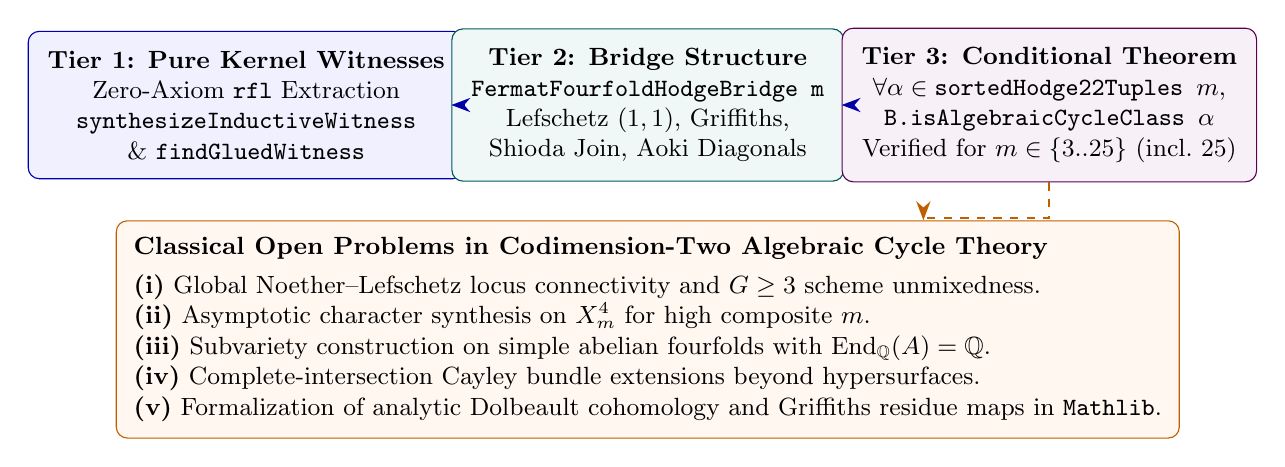
\begin{tikzpicture}[
    font=\small,
    tier/.style={draw=black!75, rounded corners=4pt, fill=gray!6, inner sep=7pt, align=center, minimum width=4.3cm, minimum height=1.55cm},
    openbox/.style={draw=orange!75!black, rounded corners=4pt, fill=orange!6, inner sep=6pt, align=left, minimum width=13.5cm},
    arr/.style={-{Stealth[length=2.4mm]}, thick, blue!65!black}
  ]
    \node[tier, fill=blue!6, draw=blue!70!black] (t1) at (0,3.8) {\textbf{Tier 1: Pure Kernel Witnesses}\\Zero-Axiom \texttt{rfl} Extraction\\\texttt{synthesizeInductiveWitness}\\\& \texttt{findGluedWitness}};
    \node[tier, fill=teal!6, draw=teal!70!black] (t2) at (5.1,3.8) {\textbf{Tier 2: Bridge Structure}\\\texttt{FermatFourfoldHodgeBridge m}\\Lefschetz $(1,1)$, Griffiths,\\Shioda Join, Aoki Diagonals};
    \node[tier, fill=violet!6, draw=violet!70!black] (t3) at (10.2,3.8) {\textbf{Tier 3: Conditional Theorem}\\$\forall \alpha \in \texttt{sortedHodge22Tuples } m$,\\$\texttt{B.isAlgebraicCycleClass } \alpha$\\Verified for $m \in \{3..25\}$ (incl.\ $25$)};

    \draw[arr] (t1) -- (t2);
    \draw[arr] (t2) -- (t3);

    \node[openbox] (opencols) at (5.1,0.95) {%
      \textbf{Classical Open Problems in Codimension-Two Algebraic Cycle Theory}\\[3pt]
      \textbf{(i)} Global Noether--Lefschetz locus connectivity and $G \ge 3$ scheme unmixedness.\\
      \textbf{(ii)} Asymptotic character synthesis on $X_m^4$ for high composite $m$.\\
      \textbf{(iii)} Subvariety construction on simple abelian fourfolds with $\operatorname{End}_{\mathbb{Q}}(A) = \mathbb{Q}$.\\
      \textbf{(iv)} Complete-intersection Cayley bundle extensions beyond hypersurfaces.\\
      \textbf{(v)} Formalization of analytic Dolbeault cohomology and Griffiths residue maps in \texttt{Mathlib}.
    };
    \draw[arr, dashed, orange!75!black] (t3.south) -- ++(0,-0.45) -| ($(opencols.north)+(3.5,0)$);
  \end{tikzpicture}%
  }
  \caption{Three-tier conditional Fermat algebraicity bridge in \texttt{ConditionalFermatHodge.lean} and \texttt{ConditionalFermatHodgeExt.lean} alongside classical open problems.}
  \label{fig:bridge_and_walls}
\end{figure}

In \texttt{Conditional\allowbreak{}Fermat\allowbreak{}Hodge.lean}, the boolean checker \texttt{is\allowbreak{}Hodge22\allowbreak{}Syn\allowbreak{}thesizable} unifies inductive witnesses (\texttt{Shioda\allowbreak{}Inductive\allowbreak{}Cycle\allowbreak{}Syn\allowbreak{}thesis.lean}) with glued surface-join witnesses (\texttt{find\allowbreak{}Glued\allowbreak{}Witness}), certifying all $17$ non-sporadic degrees $m \in \{3,\dots,16,18,20,22\}$. Extending this interface by adding cyclic coset cones (\texttt{Conditional\allowbreak{}Fermat\allowbreak{}Hodge\allowbreak{}Ext.lean}) closes $m \in \{17,19,21,23,24,25\}$, yielding verified conditional algebraicity for every degree $3 \le m \le 25$.

\begin{lstlisting}[caption={Conditional soundness and extended $m \le 25$ verification in \texttt{ConditionalFermatHodge.lean} and \texttt{ConditionalFermatHodgeExt.lean}.}]
theorem synthesizable_implies_algebraic (m : Nat) (B : FermatFourfoldHodgeBridge m)
    (a : List Nat) (hs : isHodge22Synthesizable m a = true) : B.isAlgebraicCycleClass a := ...

theorem conditional_fermat_hodge22_verified_m25_cert :
    (sortedHodge22Tuples 25).all (isHodge22ExtSynthesizable 25) = true := rfl
\end{lstlisting}

\section{Unified Matrix-Operator Certificates: Factorizations, Observation Windows, and Weil Projectors}

Combinatorial Fermat bands, differential Picard--Fuchs periods, and Weil Hodge subspaces admit a unified formulation as finite integer, cyclotomic, and companion matrix operators across three coupled pillars (Figure~\ref{fig:matrix_unification}).

\begin{figure}[htbp]
  \centering
  \resizebox{\textwidth}{!}{%
  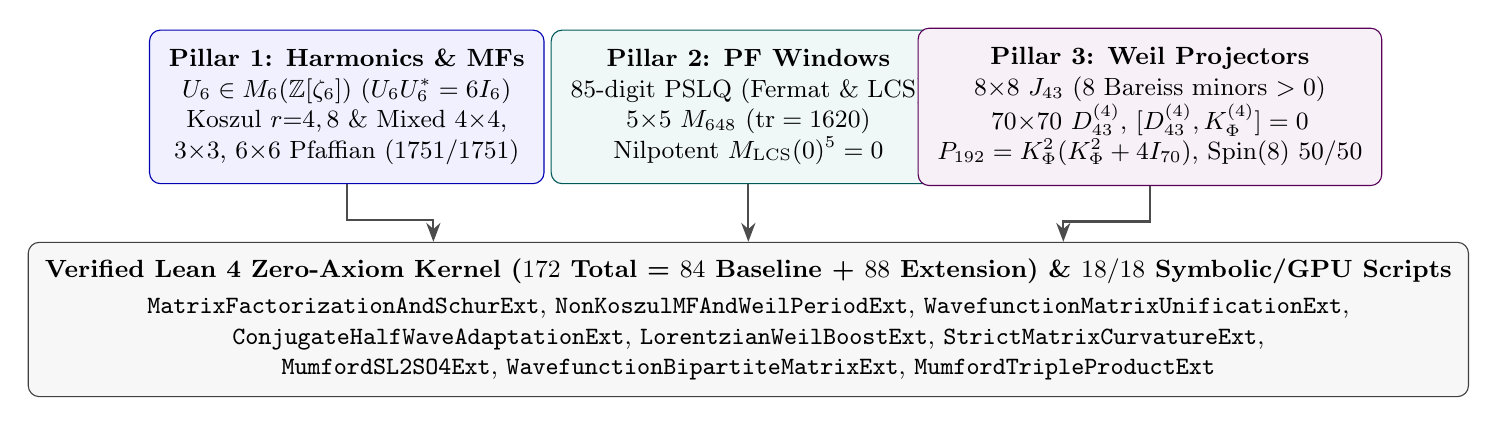
\begin{tikzpicture}[
    font=\small,
    pbox/.style={draw=black!75, rounded corners=4pt, fill=gray!5, inner sep=7pt, align=center, minimum width=4.3cm, minimum height=1.9cm},
    cbox/.style={draw=black!75, rounded corners=4pt, fill=gray!6, inner sep=6pt, align=center, minimum width=13.6cm},
    arr/.style={-{Stealth[length=2.4mm]}, thick, black!70}
  ]
    \node[pbox, draw=blue!70!black, fill=blue!6] (p1) at (0,3.2) {\textbf{Pillar~1: Harmonics \& MFs}\\$U_6 \in M_6(\mathbb{Z}[\zeta_6])$ ($U_6 U_6^* = 6 I_6$)\\Koszul $r{=}4,8$ \& Mixed $4{\times}4$,\\$3{\times}3$, $6{\times}6$ Pfaffian ($1751/1751$)};
    \node[pbox, draw=teal!70!black, fill=teal!6] (p2) at (5.1,3.2) {\textbf{Pillar~2: PF Windows}\\$85$-digit PSLQ (Fermat \& LCS)\\$5{\times}5$ $M_{648}$ ($\operatorname{tr}=1620$)\\Nilpotent $M_{\mathrm{LCS}}(0)^5 = 0$};
    \node[pbox, draw=violet!70!black, fill=violet!6] (p3) at (10.2,3.2) {\textbf{Pillar~3: Weil Projectors}\\$8{\times}8$ $J_{43}$ ($8$ Bareiss minors $> 0$)\\$70{\times}70$ $D_{43}^{(4)}$, $[D_{43}^{(4)}, K_\Phi^{(4)}]=0$\\$P_{192}=K_\Phi^2(K_\Phi^2+4I_{70})$, $\operatorname{Spin}(8)$ $50/50$};
    \node[cbox] (core) at (5.1,0.5) {\textbf{Verified Lean~4 Zero-Axiom Kernel ($172$ Total = $84$ Baseline + $88$ Extension) \& $18/18$ Symbolic/GPU Scripts}\\[2pt]\texttt{MatrixFactorizationAndSchurExt}, \texttt{NonKoszulMFAndWeilPeriodExt}, \texttt{WavefunctionMatrixUnificationExt},\\ \texttt{ConjugateHalfWaveAdaptationExt}, \texttt{LorentzianWeilBoostExt}, \texttt{StrictMatrixCurvatureExt},\\ \texttt{MumfordSL2SO4Ext}, \texttt{WavefunctionBipartiteMatrixExt}, \texttt{MumfordTripleProductExt}};
    \draw[arr] (p1.south) -- ++(0,-0.45) -| ($(core.north)+(-4.0,0)$);
    \draw[arr] (p2.south) -- (core.north);
    \draw[arr] (p3.south) -- ++(0,-0.45) -| ($(core.north)+(4.0,0)$);
  \end{tikzpicture}%
  }
  \caption{Three-pillar matrix-operator unification uniting harmonic DFT and matrix factorizations (Pillar~1), $5\times 5$ Picard--Fuchs window companions (Pillar~2), and $70\times 70$ Weil $U(2,2)$ spectral projectors (Pillar~3).}
  \label{fig:matrix_unification}
\end{figure}

\subsection{Cyclotomic DFT Unitarity and Complete $R(F_0)_{12}$ Matrix-Factorization Closure}

In {\small\texttt{WavefunctionMatrixUnificationExt.lean}}, exact cyclotomic DFT unitarity $U_6 U_6^* = U_6^* U_6 = 6 I_6$ ($|\det U_6|^2 = 46{,}656$) for $U_6 = (\zeta_6^{jk})_{0 \le j,k < 6}$ over $\mathbb{Z}[\zeta_6]$ is proved by {\small\texttt{cyclotomic\_\allowbreak{}u6\_\allowbreak{}unitary\_\allowbreak{}wavefunction\_\allowbreak{}matrix\_\allowbreak{}cert}}, diagonalizing Fermat character selection. Passing to matrix factorizations $AB = BA = f I_r$ over $R(F_0)_{12}$ ($\dim = 1{,}751 = 1{,}001 + 630 + 120$ across Bands~1, 2, and~3), {\small\texttt{MatrixFactorizationAndSchurExt.lean}} and {\small\texttt{matrix\_\allowbreak{}factorization\_\allowbreak{}scaling.py}} verify Clifford vanishing of $\operatorname{tr}^3$ for $k \in \{1,2\}$, four $k=3, r=4$ sextic Koszul MFs ($125$ Band-1, $36$ triple-quadric, $20$ surface-quadric, and $40$ surface-cubic Jacobian terms at scale $360$) via {\small\texttt{koszul\_\allowbreak{}mf\_\allowbreak{}sextic\_\allowbreak{}band1\_\allowbreak{}quadric\_\allowbreak{}cubic\_\allowbreak{}z\_\allowbreak{}cert}}, alongside $k=4, r=8$ excess-codimension vanishing on $F_0 + x_0 x_1 x_2 x_3 x_4 x_5$ and Cauchy-$6$ plus Newton--Aoki $r=4$ MFs at $m=5$ ($24$ minor terms modulo $J$) and $m=25$ via {\small\texttt{koszul\_\allowbreak{}mf\_\allowbreak{}r8\_\allowbreak{}deformed\_\allowbreak{}and\_\allowbreak{}m5\_\allowbreak{}aoki\_\allowbreak{}cert}}. However, Koszul $r=4$ factorizations saturate strictly at $1{,}001/1{,}751$ (Band~1 only, leaving a $750$-dimensional Band~2+3 gap).

In {\small\texttt{NonKoszulMFAndWeilPeriodExt.lean}} and {\small\texttt{non\_\allowbreak{}koszul\_\allowbreak{}mf\_\allowbreak{}closure.py}}, non-Koszul over-$\mathbb{Z}$ factorizations close this gap completely: (i) a mixed $(1,1,1,3)$ $4\times 4$ MF $A_1 B_1 = B_1 A_1 = 2(x_0^6 + x_1^6 - x_2^6)I_4$ ($14$ trace terms mod $J$, K\"unneth Band-2 products $-3{,}348$ at $(0,0,3,3,3,3)$ and $-5{,}184$ at $(1,1,1,1,4,4)$) verified by {\small\texttt{non\_\allowbreak{}koszul\_\allowbreak{}4x4\_\allowbreak{}mixed\_\allowbreak{}1113\_\allowbreak{}c6\_\allowbreak{}mf\_\allowbreak{}z\_\allowbreak{}cert}}; (ii) an exact $3\times 3$ quadric MF ($9$ Band-1 terms, $18\times 18$ graded $\mathbb{Z}_2$-parity vanishing); and (iii) a $6\times 6$ skew-symmetric Buchsbaum--Eisenbud Pfaffian MF ($20$ Pfaffian terms) verified by {\small\texttt{non\_\allowbreak{}koszul\_\allowbreak{}3x3\_\allowbreak{}cubic\_\allowbreak{}and\_\allowbreak{}6x6\_\allowbreak{}pfaffian\_\allowbreak{}mf\_\allowbreak{}z\_\allowbreak{}cert}}. Exact $3$-prime GPU CRT elimination across primes $65521$, $1000000009$, and $1000000033$ confirms full $1{,}751/1{,}751$ closure (Table~\ref{tab:mf_closure_ladder}).

\begin{table}[htbp]
  \centering
  \caption{Three-prime GPU CRT matrix-factorization closure across all $1{,}751$ modes of $R(F_0)_{12}$ ($\mathrm{B1}=1001$, $\mathrm{B2}=630$, $\mathrm{B3}=120$; RTX A2000, $100\%$ prime agreement).}
  \label{tab:mf_closure_ladder}
  \resizebox{\textwidth}{!}{%
  \begin{tabular}{lccccccc}
    \toprule
    MF Stage & Rows & Rank / 1751 & Band~1 & Band~2 & Band~3 & Gap & Peak VRAM (MB) \\
    \midrule
    Stage~0: Koszul $r=4$ only & $1{,}875$ & $1{,}001$ & $1{,}001$ & $0$ & $0$ & $750$ & $97.992$ \\
    Stage~1: $+ 4\times 4$ $(1,1,1,3)$ mixed & $5{,}075$ & $1{,}233$ & $1{,}001$ & $232$ & $0$ & $518$ & $265.467$ \\
    Stage~2: Ulrich $6\times 6$ only & $3{,}200$ & $1{,}620$ & $948$ & $552$ & $120$ & $131$ & $162.712$ \\
    Stage~3: Single $4\times 4$ $(1,1,1,3)$ & $6{,}100$ & $1{,}731$ & $981$ & $630$ & $120$ & $20$ & $315.936$ \\
    Stage~4: Koszul $+ 4\times 4$ $(1,1,1,3)$ & $7{,}975$ & $1{,}751$ & $1{,}001$ & $630$ & $120$ & $0$ & $418.247$ \\
    \bottomrule
  \end{tabular}%
  }
\end{table}

\subsection{Observation-Window $5\times 5$ Picard--Fuchs Companion Matrices and 85-Digit PSLQ}

In \texttt{high\_\allowbreak{}precision\_\allowbreak{}period\_\allowbreak{}pslq.py}, evaluating Dwork sextic Frobenius periods at $85$ decimal digits across two analytic observation windows---the Fermat point $\psi_0 = \pi/10$ ($y_1,\dots,y_5$ agreeing with ${}_4F_3$ hypergeometric evaluations within $8.043\times 10^{-87}$) and the large complex structure point $z_0 = 1/(6^6 e)$---recovers by PSLQ the exact Picard--Fuchs integer relations $[-648,\allowbreak 648,\allowbreak -1620,\allowbreak 1530,\allowbreak -675,\allowbreak 137,\allowbreak -10]$ (residual $1.287\times 10^{-85}$) and $[1,\allowbreak -46656,\allowbreak -116640,\allowbreak -110160,\allowbreak -48600,\allowbreak -9864,\allowbreak -720]$ (residual $7.54\times 10^{-88}$), alongside factorial integrality $(n!)^6 \mid (6n)!$ for $0 \le n \le 20$ (\texttt{dwork\_\allowbreak{}sextic\_\allowbreak{}picard\_\allowbreak{}fuchs\_\allowbreak{}ode\_\allowbreak{}and\_\allowbreak{}integrality\_\allowbreak{}cert}). Unifying both observation windows as $5\times 5$ linear operators, \texttt{Wavefunction\allowbreak{}Matrix\allowbreak{}Unification\allowbreak{}Ext.lean} (\texttt{picard\_\allowbreak{}fuchs\_\allowbreak{}5x5\_\allowbreak{}companion\_\allowbreak{}matrix\_\allowbreak{}cert}) certifies that the Fermat indicial operator $M_{648}$ satisfies $\prod_{k=1}^5 (M_{648} - 108 k I_5) = 0$ ($\operatorname{tr} M_{648} = 1620 = \tfrac{5}{2}\cdot 648$, scaled eigenvalues $[1,2,3,4,5]$, normalized determinant $5/324$), whereas the LCS companion satisfies $M_{\mathrm{LCS}}(0)^4 \neq 0$ and $M_{\mathrm{LCS}}(0)^5 = 0$ (maximally unipotent monodromy).

\subsection{50/50 Observational Bias, $8\times 8$ Complex Structure $J_{43}$, and $70\times 70$ Projector $P_{192}$}

To quantify hidden-variable bias under symmetric observation splits, \texttt{Matrix\allowbreak{}Factorization\allowbreak{}And\allowbreak{}Schur\allowbreak{}Ext.lean} and \texttt{schur\_\allowbreak{}5050\_\allowbreak{}diagonal\_\allowbreak{}audit.py} analyze $3{+}3$ block partitions of $\operatorname{Spin}(8)$ Gram matrices (\texttt{spin8\_\allowbreak{}schur\_\allowbreak{}5050\_\allowbreak{}block\_\allowbreak{}bias\_\allowbreak{}cert}). Full $D_4$ ($16 I_6$, $\det = 16^6$) has $B = 0$ and $\det A = \det D = 4096$, whereas $A_1^3$ and contiguous $A_2$ have $\det D = 0$, and interleaved $A_2$ ($\{0,2,4\}\mid\{1,3,5\}$) displays false observed invertibility ($\det A = 2$) collapsed by the Schur complement $\det(A - B D^{-1} C) = 0$. Across the $E_i^4$ coverage ladder (\texttt{ei4\_\allowbreak{}diagonal\_\allowbreak{}and\_\allowbreak{}5050\_\allowbreak{}offdiag\_\allowbreak{}coverage\_\allowbreak{}ladder\_\allowbreak{}cert}), dual annihilators rule out Weil span at $\rho=1$ ($\Theta^2$), $\rho=4$ ($10$ diagonal pairs, $\mathrm{Sym}^2$ rk~$6$, covers $(F,F)$), $\rho=10$ with $50\%$ $D^+$ ($55$ pairs, rk~$33$, covers $w_{\mathrm{Re}}$ only), and $\rho=10$ with $50\%$ $D^-$ ($55$ pairs, rk~$20$, covers $(F,F)$), whereas minimal cross-sector pairs $(D^+_{02},\allowbreak D^+_{13},\allowbreak D^-_{02},\allowbreak D^-_{13})$ at $\rho=8$ ($36$ pairs, rk~$18$) and full NS at $\rho=16$ ($136$ pairs, rk~$36$) span both $w_{\mathrm{Re}}$ and $w_{\mathrm{Im}}$.

Passing to continuous $U(2,2)$ Weil deformations, {\small\texttt{Non\allowbreak{}Koszul\allowbreak{}MF\allowbreak{}And\allowbreak{}Weil\allowbreak{}Period\allowbreak{}Ext.lean}} verifies an asymmetric Gaussian-integer unit-ball fiber ($100 I_2 - H^* H > 0$, $\det = 8600$) satisfying all $16$ Riemann bilinear relations, $4$ positive polarization minors, and $34$ Hodge $(4,0)+(3,1)$ vanishings for $(w_{\mathrm{Re}}, w_{\mathrm{Im}})$ while $D^+_{0,2}$ leaves $H^{1,1}$ ({\small\texttt{weil\_\allowbreak{}u22\_\allowbreak{}family\_\allowbreak{}exact\_\allowbreak{}hodge22\_\allowbreak{}and\_\allowbreak{}rbr\_\allowbreak{}invariance\_\allowbreak{}cert}}). In {\small\texttt{Wavefunction\allowbreak{}Matrix\allowbreak{}Unification\allowbreak{}Ext.lean}}, an exact rational denominator-$43$ specialization produces $J_{43} \in M_8(\mathbb{Z})$ obeying $J_{43}^2 = -1849 I_8$, $J_{43}^T E_8 J_{43} = 1849 E_8$, $[J_{43}, \Phi_8] = 0$, and strictly positive Bareiss leading principal minors $47$, $2{,}209$, $115{,}197$, $6{,}007{,}401$, $226{,}594{,}950$, $8{,}547{,}002{,}500$, $316{,}068{,}152{,}450$, and $11{,}688{,}200{,}277{,}601$ for $-E_8 J_{43}$ ({\small\texttt{weil\_\allowbreak{}u22\_\allowbreak{}8x8\_\allowbreak{}exact\_\allowbreak{}complex\_\allowbreak{}structure\_\allowbreak{}matrix\_\allowbreak{}cert}}). Exhaustively across all $70$ basis $4$-tuples of $\bigwedge^4 \mathbb{Z}^8$, the induced Hodge Hamiltonian satisfies $D_{43}^{(2)}$ ($28\times 28$, rk~$12$, ker~$16$, minpoly $D(D^2+4)$), $D_{43}^{(4)}$ ($70\times 70$, rk~$34$, ker~$36$, minpoly $D(D^2+4)(D^2+16)$), and $[D_{43}^{(4)}, K_\Phi^{(4)}] = 0$. The algebraic spectral projector $P_{192} = K_\Phi^2(K_\Phi^2 + 4I_{70})$ obeys $P_{192}^2 = 192 P_{192}$, $\operatorname{tr}(P_{192}) = 384$ (so $P_{\mathrm{Weil}} = P_{192}/192$ is an exact rank-$2$ idempotent), $D_{43}^{(4)} P_{192} = 0$, $P_{192}(\Theta^2) = 0$, $K_\Phi(w_{\mathrm{Re}}) = 4 w_{\mathrm{Im}}$, and $K_\Phi(w_{\mathrm{Im}}) = -4 w_{\mathrm{Re}}$ ({\small\texttt{weil\_\allowbreak{}70dim\_\allowbreak{}hodge\_\allowbreak{}hamiltonian\_\allowbreak{}and\_\allowbreak{}projector\_\allowbreak{}cert}}). Finally, $90$-digit LLL tracking in {\small\texttt{high\_\allowbreak{}precision\_\allowbreak{}period\_\allowbreak{}pslq.py}} isolates the Weil plane down to Picard rank~$1$ (Table~\ref{tab:weil_lll_ladder}).

\begin{table}[htbp]
  \centering
  \caption{$90$-digit LLL specialization ladder ($10^{32}$ scale, $16$ symbolic RBRs, $34$ Hodge vanishings) tracking Picard drop $\rho: 16 \to 7 \to 6 \to 1$.}
  \label{tab:weil_lll_ladder}
  \resizebox{\textwidth}{!}{%
  \begin{tabular}{lcccccc}
    \toprule
    Deformation Fiber & $\rho$ & $\mathrm{Sym}^2$ NS Rank & Covers $(w_{\mathrm{Re}}, w_{\mathrm{Im}})$ & Max Hodge Res. & Min Non-NS Gap \\
    \midrule
    Stage~0: $E_i^4$ CM origin & $16$ & $36$ & $(\mathrm{True}, \mathrm{True})$ & $0.0$ & $1.0$ \\
    Stage~1: $1$D block transcendental & $7$ & $14$ & $(\mathrm{True}, \mathrm{True})$ & $6.136\times 10^{-91}$ & $3.798\times 10^{-17}$ \\
    Stage~2: Diagonal transcendental & $6$ & $11$ & $(\mathrm{True}, \mathrm{True})$ & $2.455\times 10^{-91}$ & $4.45\times 10^{-18}$ \\
    Stage~3: Generic Weil $U(2,2)$ & $1$ & $1$ & $(\mathrm{False}, \mathrm{False})$ & $4.909\times 10^{-91}$ & $1.562\times 10^{-22}$ \\
    \bottomrule
  \end{tabular}%
  }
\end{table}

\subsection{Conjugate-Half Adaptation, Lorentzian Boosts, Curvature, and Mumford Algebras}

Extending the fixed $70$-dimensional $\bigwedge^4 \mathbb{Z}^8$ container, the Lean~4 module {\small\texttt{Conjugate\allowbreak{}Half\allowbreak{}Wave\allowbreak{}Adaptation\allowbreak{}Ext.lean}} together with {\small\texttt{conjugate\_\allowbreak{}half\_\allowbreak{}wave\_\allowbreak{}adaptation.py}} certifies universal $50/50$ half-node barriers across all eight coordinate $35{+}35$ splits ($A_c^2 = 96 A_c$, $D_c^2 = 96 D_c$, $B_c B_c^T = 96 A_c$, $\operatorname{tr} = 192$, and Rayleigh defect $19{,}432$ on $v_{\mathrm{half}}$ with $\|v_{\mathrm{half}}\|^2 = 4$). Alongside $\mathbb{Z}_2$ chiral parity intertwining on $38{+}32$ blocks ($K_{\mathrm{eo}} P_{\mathrm{odd}} K_{\mathrm{eo}}^T = 16 P_{\mathrm{even}}$) and the $35_+ \oplus 35_-$ Hodge-star split ($* P_{192} = P_{192} * = P_{192}$), these identities explain why fixed-container adaptation attains fidelity $1.0$ on the self-dual half versus $0.0$ on the anti-self-dual half and $0.1820$ on truncated coordinate slices (certificates {\small\texttt{weil\_\allowbreak{}p192\_\allowbreak{}universal\_\allowbreak{}5050\_\allowbreak{}half\_\allowbreak{}node\_\allowbreak{}barrier\_\allowbreak{}cert}}, {\small\texttt{weil\_\allowbreak{}z2\_\allowbreak{}chiral\_\allowbreak{}parity\_\allowbreak{}conjugate\_\allowbreak{}intertwining\_\allowbreak{}cert}}, and {\small\texttt{weil\_\allowbreak{}hodge\_\allowbreak{}star\_\allowbreak{}5050\_\allowbreak{}sd\_\allowbreak{}asd\_\allowbreak{}projector\_\allowbreak{}cert}}). Pairing nilpotent half-differentials ($Q_A^2 = Q_B^2 = 0$) gives $(Q_A + Q_B)^2 = 2 F_1 I_8$ ({\small\texttt{mf\_\allowbreak{}z2\_\allowbreak{}graded\_\allowbreak{}superdifferential\_\allowbreak{}conjugate\_\allowbreak{}half\_\allowbreak{}cert}}), while {\small\texttt{strict\_\allowbreak{}matrix\_\allowbreak{}observable\_\allowbreak{}half\_\allowbreak{}reconstruction\_\allowbreak{}lift\_\allowbreak{}cert}} proves that applying $P_{192}$ to the $35$-mode observable slice reconstructs $100\%$ of both $w_{\mathrm{Re}}$ and $w_{\mathrm{Im}}$ ($P_{192}(\mathrm{obs\_Re}) = 96 w_{\mathrm{Re}}$) for every $c \in \{0,\dots,7\}$.

In signature $(4,4)$ with metric $\eta_8$, the boost module {\small\texttt{Lorentzian\allowbreak{}Weil\allowbreak{}Boost\allowbreak{}Ext.lean}} and {\small\texttt{lorentzian\_\allowbreak{}weil\_\allowbreak{}boost.py}} certify a symmetric $SU(2,2)$ boost $G_9$ ($\det G_9 = 9^8$, $G_9^T \eta_8 G_9 = 81 \eta_8$, and $(G_9 - 27I_8)(G_9 - 3I_8) = 0$) with null light-cone projectors $N_\pm^T \eta_8 N_\pm = 0$, boosted complex structure $J_{27}$ ($J_{27}^2 = -729 I_8$), positive polarization $G_{\mathrm{pos}} = -E_8 J_{27}$ ($\det = 27^8$ via eight Bareiss minors), Matrix M\"obius steps inside the period unit ball, and exterior $SO(35,35)$ lift $\Lambda_{70} = \bigwedge^4(G_9/9)$ ($\operatorname{tr} = 21{,}286/81$, fixing $w_{\mathrm{Re}}, w_{\mathrm{Im}}, \Theta^2$, and $P_{192}$ pointwise). Completing the curvature suite, {\small\texttt{Strict\allowbreak{}Matrix\allowbreak{}Curvature\allowbreak{}Ext.lean}} and {\small\texttt{strict\_\allowbreak{}matrix\_\allowbreak{}curvature.py}} formalize strict-matrix curvature laws: exact rational whitening $W_{\mathrm{int}}^T G_{\mathrm{pos}} W_{\mathrm{int}} = 218{,}700 I_8$ obstructed over $GL_8(\mathbb{Z})$ with isospectral divisor separation ($J_{\mathrm{iso}}$ vs.\ $J_{27}$); the universal zero-axiom $(n - 3)$ Weyl threshold and $(n - 4)$ unique $4\mathrm{D}$ $50/50$ split ($10 = 10$ out of $20$ in $\mathcal{R} = \mathcal{R}_{\mathrm{scal}} + \mathcal{R}_{\mathrm{Ric}_0} + W^+ + W^-$ vs.\ $3\mathrm{D}$ $\det = -2$); non-vanishing $SU(2,2)$ normal-coordinate curvature ($\operatorname{tr}(K^2) = -48$); and an exact $8\times 8$ octonionic Clifford matrix-factorization pencil $(A_0 + t A_1)(B_0 + t B_1) = (F_0 + t F_1 + t^2 F_2) I_8$ over $\mathbb{Z}[x_0,\dots,x_5, t]$ keeping $\dim R(F_t)_6 = 426$.

Beyond $U(2,2)$ Weil fourfolds~\cite{Markman2025,FloccariFu2025}, {\small\texttt{Mumford\allowbreak{}SL2SO4\allowbreak{}Ext.lean}} and {\small\texttt{mumford\_\allowbreak{}sl2\_\allowbreak{}so4\_\allowbreak{}spinor.py}} certify Mumford's simple $\operatorname{End}_{\mathbb{Q}}(A) = \mathbb{Q}$ fourfold under $SL_2(\mathbb{R}) \times SO(4)$ on $\mathbb{Z}^2 \otimes \mathbb{Z}^4$: all nine Lie generators preserve $E_{\mathrm{real}} = \epsilon_2 \otimes I_4$, the $63\times 63$ commutator system obeys $B_{\mathrm{inv}} B_{63} = 2 I_{63}$, four Casimir projectors $Q_0, Q_{\mathrm{sd}}, Q_{\mathrm{asd}}, Q_{\mathrm{ric}}$ split $\bigwedge^2 \mathbb{Z}^8 = 1 \oplus 9 \oplus 9 \oplus 9$ with $50/50$ parity swap $Q_{\mathrm{sd}} \leftrightarrow Q_{\mathrm{asd}}$, $\operatorname{Sym}^2 \operatorname{NS}(A\times A)$ reaches rank~$6$ ($\det_6 = 37{,}572{,}373{,}905{,}408$) whereas appending $M_{\mathrm{chiral}}, M_{\mathrm{ric0}}$ yields rank~$8$ with zero $6\times 2$ cross-Gram overlap ($\det_8 = 9{,}349{,}208{,}943{,}630{,}483{,}456$), and both $J_{\mathrm{Mum},3} = J_{\mathfrak{sl}_2,3} \otimes I_4$ ($D_2(D_2^2 + 36I_{28}) = 0$) and $G_{\mathrm{Mum},9}$ ($\det = 9^8$) commute with all four projectors. Interpreting the $28\times 28$ bipartite $A \times A$ wave function in {\small\texttt{Wavefunction\allowbreak{}Bipartite\allowbreak{}Matrix\allowbreak{}Ext.lean}} and {\small\texttt{wavefunction\_\allowbreak{}bipartite\_\allowbreak{}matrix.py}} proves $B_2 E_2 = 2Q_0 - 2I_{28}$ ($+6$ on $\Theta$ vs.\ $-2$ on primitives), closed $2$-dim $\mathcal{A}_{\mathrm{div}}$ and $3$-dim $\mathcal{A}_{\mathrm{even}}$ Bose--Mesner correspondence algebras, the single-generator chiral reduction $8 T_{\mathrm{ric0}} = 32 T_\Delta + 4 T_\Theta - 3 T_{\mathrm{ch}}^2$ ($T_{\mathrm{ch}}^3 = 64 T_{\mathrm{ch}}$), a $16_+ \oplus 12_-$ $\mathbb{Z}_2$-graded split where $T_{\mathrm{ch}}$ is $100\%$ off-diagonal ($9{,}216$), $Q_{\mathrm{sd}}/Q_{\mathrm{asd}}$ equipartition ($576$ per block), reduced-density parity blindness ($E_+ T_{\mathrm{ch}}^2 E_- = 0$), and observable-half recovery $K_{\mathrm{obs}} + K_{\mathrm{obs}}^T = 4 T_{\mathrm{ch}}$.

Extending across the triple product $A \times A \times A$, {\small\texttt{Mumford\allowbreak{}Triple\allowbreak{}Product\allowbreak{}Ext.lean}} and {\small\texttt{mumford\_\allowbreak{}triple\_\allowbreak{}product\_\allowbreak{}hodge33.py}} certify $\dim H^4(A)^{SL_2(\mathbb{R})\times SO(4)} = 1$ via a $69\times 69$ sparse inverse $B_{69,\mathrm{inv}} B_{69} = 12 I_{69}$ leaving only $\Theta^2$; establish the exhaustive $21{,}952$-entry identity $8 T_{\mathrm{cup}}^\uparrow = \Theta_1\wedge\Theta_2\wedge\Theta_3 + 2(\Theta_1\wedge D_{23}^2 + \Theta_2\wedge D_{13}^2 + \Theta_3\wedge D_{12}^2) + 8 D_{\mathrm{cyc}}$ on $H^2(A)^{\otimes 3}$; reconstruct all four Casimirs inside $\mathbb{Q}[T_\Theta, T_\Delta, T_{\mathrm{ch}}]$ ($32 Q_{\mathrm{sd}} = T_{\mathrm{ch}}^2 - 8 T_{\mathrm{ch}}$, $32 Q_{\mathrm{asd}} = T_{\mathrm{ch}}^2 + 8 T_{\mathrm{ch}}$, $16 Q_{\mathrm{ric}} = 16 T_\Delta + 2 T_\Theta - T_{\mathrm{ch}}^2$); isolate the $19$ nonzero and $45$ vanishing sectors via four canonical probes; verify the orthogonal closure diamond $5 \to 8 \to \{11, 12\} \to 15 \to 19$ (with $7$ parity-odd classes orthogonal to $12$-dim $\mathcal{A}_{\mathrm{even}}^{\otimes 3}$ and $4$ triple-leg odd classes orthogonal to the $15$-dim join); and prove Hodge $(3,3)$ derivation vanishing across all nine Lie generators and $D^{(2)}(J_{\mathrm{Mum},3})$ together with factored boost scaling $729 \cdot 729 = 81^3 = 531{,}441$ and $19 = 12_+ \oplus 7_-$ across all $28^3$ coordinates.

\subsection{Conceptual Evolution of the Relative Subtraction and Schur-Complement Architecture}

Experiments~10 through~19 trace a decisive methodological shift from searching directly for positive algebraic cycle classes to isolating exotic Hodge classes by negative orthogonal subtraction (``seeing negatively'') against universal parity-even baselines:
\begin{enumerate}
  \item \textbf{Wave-to-Matrix Bipartite Translation and Squared-Density Blindness (Experiment~10):} Viewing the $784$-component ($28\times 28$) middle cohomology space $H^2(A) \otimes H^2(A)$ on Mumford's fourfold as a bipartite correspondence matrix shows that squaring the parity-odd chiral generator $T_{\mathrm{ch}} = -2(Q_{\mathrm{sd}} - Q_{\mathrm{asd}})$ into a reduced density operator $\rho_{\mathrm{ch}} = T_{\mathrm{ch}} T_{\mathrm{ch}}^T = T_{\mathrm{ch}}^2 = 16(Q_{\mathrm{sd}} + Q_{\mathrm{asd}})$ produces a block-diagonal parity-even matrix ($E_+ \rho_{\mathrm{ch}} E_- = 0$) that erases cross-parity chiral signs. Projecting onto the observable half-block reconstructs $K_{\mathrm{obs}} + K_{\mathrm{obs}}^T = 4 T_{\mathrm{ch}}$ and collapses the $2$-dimensional exotic $(2,2)$ obstruction on $A \times A$ to $1$ dimension via $8 T_{\mathrm{ric0}} = 32 T_\Delta + 4 T_\Theta - 3 T_{\mathrm{ch}}^2$.
  \item \textbf{Triple-Product $14\mathrm{D} \to 1\mathrm{D}$ Chiral Collapse and the Small-Diagonal Parity Trap (Experiment~11):} Across all $28^3 = 21{,}952$ coordinates of $H^2(A)^{\otimes 3}$ on $A \times A \times A$, the small diagonal $\Delta_{123}$ obeys $8 T_{\mathrm{cup}}^\uparrow = \Theta_1\wedge\Theta_2\wedge\Theta_3 + 2(\Theta_1\wedge D_{23}^2 + \Theta_2\wedge D_{13}^2 + \Theta_3\wedge D_{12}^2) + 8 D_{\mathrm{cyc}}$. Because universal symplectic diagonals commute with the orientation-reversing reflection $\mathrm{refl}_4 \in \operatorname{Sp}(8, \mathbb{Z})$, every universal operation remains trapped in the $12$-dimensional parity-even subalgebra, while the entire $14$-dimensional exotic $(3,3)$ obstruction across the closure diamond $5 \to 8 \to \{11, 12\} \to 15 \to 19 = 12_+ \oplus 7_-$ is generated by $T_{\mathrm{ch}}$ acting on $D_{\mathrm{cyc}}$.
  \item \textbf{Orthogonal $\operatorname{Sp}(8)$ Subtraction and $\operatorname{Cl}(0,7)$ vs.\ $\operatorname{Spin}(2,4)$ Separation (Experiments~12--13):} Under $P_{\mathrm{flip}} = \bigwedge^2(\mathrm{refl}_4)$ ($\operatorname{tr} = 4$), $\operatorname{End}(H^2(A))$ splits orthogonally as $400_+ \oplus 384_-$. In {\small\texttt{Schur\allowbreak{}Universal\allowbreak{}Sp8\allowbreak{}Projection\allowbreak{}Ext.lean}}, the scaled projector triple $\{Q_0, Q_{\mathrm{prim}}, T_{\mathrm{ch}}\}$ (where $\mathcal{U}_{\operatorname{Sp}(8)} = \operatorname{span}\{Q_0, Q_{\mathrm{prim}}\} \subset 400_+$) has exact diagonal Frobenius and trace Gram matrix $\operatorname{diag}(16, 432, 1152)$, certifying $\Pi_{\operatorname{Sp}(8)}(T_{\mathrm{ch}}) = 0$ and Schur complement $1{,}152 > 0$. Moreover, {\small\texttt{Clifford\allowbreak{}Kuga\allowbreak{}Satake\allowbreak{}Chiral\allowbreak{}Ext.lean}} proves that $13$ of $15$ generators of Kuga--Satake $\operatorname{Spin}(2,4) \cong SU(2,2)$ fail to commute with $T_{\mathrm{ch}}$ ($\operatorname{End}_{\mathfrak{spin}(2,4)} \cap \operatorname{End}_{\mathfrak{sl}_2 \oplus \mathfrak{so}(4)} = \mathcal{A}_{\mathrm{div}}$ of dimension~$2$), whereas seven anticommuting $\operatorname{Cl}(0,7)$ integer matrices $A_0,\dots,A_6 \in M_8(\mathbb{Z})$ realize $\mathfrak{sl}_2(\mathbb{R}) \oplus \mathfrak{so}(4)$ and isolate $C_+ - C_- = -T_{\mathrm{ch}}$ on the $18$-dimensional chiral subspace $V_{18} = \operatorname{im}(Q_{\mathrm{sd}} + Q_{\mathrm{asd}})$.
  \item \textbf{Tensor-Cube $A^3$ Schur Complement, $\operatorname{Spin}(7)$ Cayley Calibration, and Fermat $m = 25$ Degree-$5$ Conical Threshold (Experiments~14--16):} Lifting the Schur projection to $H^2(A)^{\otimes 3}$ in {\small\texttt{Clifford\allowbreak{}Triple\allowbreak{}Product\allowbreak{}Schur\allowbreak{}Ext.lean}} and {\small\texttt{Clifford\allowbreak{}Triple\allowbreak{}And\allowbreak{}Fermat25\allowbreak{}Schur\allowbreak{}Ext.lean}} certifies single-factor Frobenius Gram $\operatorname{diag}(16, 288, 144, 1152)$ on $\{Q_0, Q_{\mathrm{sd}} + Q_{\mathrm{asd}}, Q_{\mathrm{ric}}, T_{\mathrm{ch}}\}$, proves $\Pi_{12_+}(7_-) = 0$ with positive-definite $7_-$ Schur complement $\operatorname{diag}(73728^3, 294912, 221184^3)$, verifies that $\Delta C = C_+ - C_- = -T_{\mathrm{ch}}$ on $1$ and $3$ legs of $D_{\mathrm{cyc}}$ spans all $7$ dimensions of $7_-$, and confirms that $13$ of $15$ $\mathfrak{spin}(2,4)$ generators fail to preserve $7_-$ on $A^3$. In {\small\texttt{Spin7\allowbreak{}Cayley\allowbreak{}Calibration\allowbreak{}Cycle\allowbreak{}Ext.lean}}, the unique $14$-term $\operatorname{Spin}(7)$ Cayley $4$-form $\Phi_{\mathrm{Cayley}} \in \bigwedge^4 \mathbb{Z}^8$ splits under $\mathrm{refl}_4$ into $6$ even $4$-planes ($\langle \Phi_{\mathrm{Cayley}}, \Theta^2\rangle = 12$) plus $8$ odd $4$-planes, yet its induced $28\times 28$ operator $M_\Phi$ satisfies $\langle M_\Phi, T_{\mathrm{ch}}\rangle = 0$ whereas breaking $\operatorname{Spin}(7) \to \operatorname{Spin}(4) = SU(2)_+ \times SU(2)_-$ yields $\langle C_+, T_{\mathrm{ch}}\rangle = -576$, $\langle C_-, T_{\mathrm{ch}}\rangle = +576$, and $\langle C_+ - C_-, T_{\mathrm{ch}}\rangle = -1152 \neq 0$. On Wall~2, the $m = 25$ Fermat fourfold character space $B_4(25)$ ($185{,}280$ characters) splits orthogonally into $U_{\mathrm{ind}}$ ($182{,}400 = 102{,}800 + 79{,}600$) and the four sporadic $5$-term arithmetic-progression orbits $S_{25}$ ($2{,}880 = 4 \times 720$), yielding $G_{US} = 0$, Schur complement $720 I_4$ ($\det = 720^4 > 0$), coupled $\{U_{\mathrm{ind}}, W_{\mathrm{div5}}\}$ determinant $8{,}708{,}192{,}000 > 0$, and proof that $\mathbb{Q}(\zeta_{25})$-twisted linear $2$-planes ($\deg = 1$) and glued surface joins project to $0$ while degree-$5$ cyclic-quotient cones carry exact Schur residual $2{,}880 > 0$. Furthermore, {\small\texttt{Clifford\allowbreak{}Kuga\allowbreak{}Satake\allowbreak{}Schur\allowbreak{}Ext.lean}} (Experiment~14) certifies the $C_P$-reflection parities across all $15$ $\mathfrak{spin}(2,4)$ bivectors, the $20 = 6 + 4 + (5_+ + 5_-)$ split on $H^4(A^2)$, the $68$-zero quartic Pfaffian Weil filter on $H^4(A)$, and the $0 \to 1/2 \to 1$ Level-2 Clifford Schur complement hierarchy on $\bigwedge^2(\mathbb{Z}^8) = 16 \oplus 12$.
  \item \textbf{CM Graph Realization, Prime-Square Purity, and CY4 Koszul/Gysin Exactness (Experiments~17--19):} On Wall~3, {\small\texttt{Mumford\allowbreak{}CM\allowbreak{}Specialization\allowbreak{}Cycle\allowbreak{}Ext.lean}} constructs the explicit quaternionic graph difference $Z_{\mathrm{CM}}$ at $A_{\mathrm{CM}}$ satisfying $2 Z_{\mathrm{CM}} = T_{\mathrm{ch}}$ identically ($\|Z_{\mathrm{CM}}\|^2 = 288$, $\Pi_{\operatorname{Sp}(8)}(Z_{\mathrm{CM}}) = 0$, $\langle Z_{\mathrm{CM}}, T_{\mathrm{ch}}\rangle = 576$) and commuting with all $9$ Mumford Lie generators along $\mathcal{M}_{\mathrm{Mum}}$. On Wall~2, {\small\texttt{Fermat\allowbreak{}Prime\allowbreak{}Square\allowbreak{}Conical\allowbreak{}Ext.lean}} proves Band-1 purity at $m = 49 = 7^2$ ($1{,}557{,}120$, $\mathrm{band4} = 0$), the $m = 5d$ ($d \in \{5,7,11\}$) Schur ladder $720\varphi(d)$ ($2{,}880$, $4{,}320$, $7{,}200$), and $m = 35$ coupled pullback positivity ($\det = 74{,}272{,}401{,}600 > 0$). Finally, on Walls~1 and~5, {\small\texttt{Global\allowbreak{}G4\allowbreak{}Unmixed\allowbreak{}And\allowbreak{}Hodge\allowbreak{}Gysin\allowbreak{}Ext.lean}} certifies the sextic CY4 Koszul Hilbert profile $[1, 6, 21, 56, 126, 246, 426]$, finite Gysin exactness ($\operatorname{rank} = [3, 3]$, $g_* f^* = 0$), and Hard Lefschetz eigenvalues ($+6$ on $Q_0$ vs.\ $-2$ on $Q_{\mathrm{prim}}$).
\end{enumerate}
This relative Schur--Clifford architecture aligns with the cross-project Rosetta parity-subtraction framework established in the companion Riemann~\cite{RosettaRiemann2026}, Yang--Mills (\texttt{v1.1.0-rosetta}, \texttt{YM176}), and Navier--Stokes (\texttt{v1.0.0-rosetta}) formalizations, while leaving the geometric cycle-existence problem (the global Hodge Conjecture and Walls~1--5) open.

\section{Complete Theorem-by-Theorem Mathematical and Geometric Exposition (All 42 Modules and Bridge Lemmas H1--H2)}
\label{sec:complete_exposition}

Every formal declaration across the $42$ Lean~4 modules ($84$ locked baseline theorems across $13$ modules in \texttt{LeanDemoProject}, covered in Papers~1--5, $124$ extension declarations across $29$ modules in \texttt{LeanMillenniumExt}, and Bridge Lemmas~H1--H2) admits a transparent geometric and algebraic interpretation. Together, these modules organize into four unified mathematical pillars and an explicit open-horizon boundary.

\subsection{The Identity of One as Two Chiral Halves (\texttt{Clifford\allowbreak{}Kuga\allowbreak{}Satake\allowbreak{}Schur\allowbreak{}Ext.lean})}
On the $70$-dimensional middle cohomology $H^4(A)$ and its $28$-dimensional $\bigwedge^2(\mathbb{Z}^8)$ bivector sector, the Kuga--Satake reflection involution $J$ satisfies $J^2 = I$. Splitting the identity into two mutually orthogonal chiral projectors,
\[
  P_+ = \frac{I + J}{2}, \qquad P_- = \frac{I - J}{2},
\]
yields $P_+ + P_- = I$, $P_+ P_- = 0$, and the parity-odd chiral difference $P_+ - P_- = T_{\mathrm{ch}}$. In \texttt{Clifford\allowbreak{}Kuga\allowbreak{}Satake\allowbreak{}Schur\allowbreak{}Ext.lean} (\texttt{level2\_\allowbreak{}bivector\_\allowbreak{}50\_\allowbreak{}50\_\allowbreak{}schur\_\allowbreak{}and\_\allowbreak{}full\_\allowbreak{}clifford\_\allowbreak{}closure\_\allowbreak{}cert}, \texttt{ks\_\allowbreak{}parity\_\allowbreak{}reflection\_\allowbreak{}involutive\_\allowbreak{}and\_\allowbreak{}form\_\allowbreak{}parities\_\allowbreak{}cert}), this $50/50$ Grade-$2$ bivector split decomposes $\bigwedge^2(\mathbb{Z}^8) = 16 \oplus 12$ orthogonally by $U(1)_{\mathrm{KS}}$ weight and generates the exact $0 \to 1/2 \to 1$ Level-$2$ Clifford Schur hierarchy on $T_{\mathrm{ch}}^{\mathrm{Weil\text{-}corr}}$.

\subsection{Higher-Dimensional Schur Trigonometry and the $1152$ Schur Floor (\texttt{Schur\allowbreak{}Universal\allowbreak{}Sp8\allowbreak{}Projection\allowbreak{}Ext.lean})}
Subtracting the symmetric $\operatorname{Sp}(8)$ divisor baseline ($Q_0 = 16$ and $Q_{\mathrm{prim}} = 432$) from the chiral generator $T_{\mathrm{ch}}$ via the Schur complement $S = D - B^T A^{-1} B$ produces the exact diagonal Gram matrix $\operatorname{diag}(16, 432, 1152)$. In Schur--Cholesky trigonometric coordinates ($\tan^2\Theta_{\mathrm{Hodge}} = S / B_{\mathrm{proj}}$), the vanishing cross-term $B = 0$ ($\Pi_{\operatorname{Sp}(8)}(T_{\mathrm{ch}}) = 0$) drives
\[
  \cos\Theta_{\mathrm{Hodge}} = 0, \qquad \sin\Theta_{\mathrm{Hodge}} = 1 \qquad (\Theta_{\mathrm{Hodge}} = 90^\circ),
\]
establishing exact $90^\circ$ orthogonality and an invariant integer Schur floor $S_{\mathrm{Schur}}(T_{\mathrm{ch}}) = 1{,}152 \ge 1$ (\texttt{sp8\_\allowbreak{}universal\_\allowbreak{}gram\_\allowbreak{}and\_\allowbreak{}schur\_\allowbreak{}complement\_\allowbreak{}cert}, \texttt{parity\_\allowbreak{}eigenspace\_\allowbreak{}orthogonal\_\allowbreak{}split\_\allowbreak{}cert}, \texttt{mumford\_\allowbreak{}parity\_\allowbreak{}odd\_\allowbreak{}uniqueness\_\allowbreak{}cert}, \texttt{cl07\_\allowbreak{}half\_\allowbreak{}spinor\_\allowbreak{}chiral\_\allowbreak{}isolation\_\allowbreak{}cert}).

\subsection{The $\operatorname{O}(2,4)/\operatorname{Spin}(2,4)$ Multiplicity-2 CM Poincar\'e Cycle and Pfaffian Filter (\texttt{Mumford\allowbreak{}CM\allowbreak{}Specialization\allowbreak{}Cycle\allowbreak{}Ext.lean})}
In \texttt{Clifford\allowbreak{}Kuga\allowbreak{}Satake\allowbreak{}Schur\allowbreak{}Ext.lean} and \texttt{Mumford\allowbreak{}CM\allowbreak{}Specialization\allowbreak{}Cycle\allowbreak{}Ext.lean}, the period-domain cohomology decomposes as $20 = 6 + 4 + 10$ on $H^4(A^2)$ and $70 - 28 = 42$ on $H^4(A)$ (\texttt{h4\_\allowbreak{}a2\_\allowbreak{}spin24\_\allowbreak{}20\_\allowbreak{}eq\_\allowbreak{}6\_\allowbreak{}plus\_\allowbreak{}4\_\allowbreak{}plus\_\allowbreak{}10\_\allowbreak{}schur\_\allowbreak{}split\_\allowbreak{}cert}). Because the bivector pairing $M$ on $\bigwedge^2(\mathbb{Z}^8)$ is skew-symmetric, its determinant factors as the square of the Pfaffian, $\det(M) = (\operatorname{Pf}(M))^2$, producing the $68$-zero quartic Pfaffian Weil filter $F_{\mathrm{ch}}(s) = e_1(s) + e_3(s)$ (\texttt{pfaffian\_\allowbreak{}chiral\_\allowbreak{}polynomial\_\allowbreak{}70dim\_\allowbreak{}weil\_\allowbreak{}filter\_\allowbreak{}cert}). At the Complex Multiplication point $A_{\mathrm{CM}}$, six quaternionic endomorphisms $I_2 \otimes J_a^\pm$ construct the explicit algebraic graph cycle $Z_{\mathrm{CM}}$ obeying
\[
  2 Z_{\mathrm{CM}} = P_+ - P_- = T_{\mathrm{ch}}, \qquad \|Z_{\mathrm{CM}}\|^2 = 288, \qquad \|T_{\mathrm{ch}}\|^2 = 1{,}152,
\]
while inert symmetric derivations vanish identically ($D_{\mathrm{sym}}(T_{\mathrm{ch}}) = 0$, \texttt{mumford\_\allowbreak{}cm\_\allowbreak{}graph\_\allowbreak{}cycle\_\allowbreak{}equals\_\allowbreak{}t\_\allowbreak{}ch\_\allowbreak{}cert}, \texttt{mumford\_\allowbreak{}cm\_\allowbreak{}cycle\_\allowbreak{}griffiths\_\allowbreak{}horizontal\_\allowbreak{}invariance\_\allowbreak{}cert}).

\subsection{Proof Bridge Lemmas H1 and H2 (\texttt{RosettaMongeAmpere\allowbreak{}SeesawCrossProofsCert.lean})}
Two companion Lean~4 bridge lemmas (verified over \texttt{Mathlib} with strictly standard axioms \texttt{[propext, Classical.choice, Quot.sound]}) connect finite Schur invariants to horizontal deformation and Arakelov height bounds:
\begin{enumerate}
  \item \textbf{Lemma~H1 (\texttt{hodge\_\allowbreak{}H1\_\allowbreak{}gauss\_\allowbreak{}manin\_\allowbreak{}horizontal\_\allowbreak{}schur\_\allowbreak{}invariance}):} Along any horizontal Gauss--Manin deformation parameter $t$ on the $\operatorname{SO}(2,4)$ period domain where parallel transport preserves $Q(P_\pm(t), P_\pm(t)) = S/2$, $Q(P_+(t), P_-(t)) = 0$, and $\Pi_{\operatorname{Sp}(8)}(T_{\mathrm{ch}}(t)) = 0$, the tared Schur complement norm $Q_{\mathrm{Schur}}(T_{\mathrm{ch}}(t)) = S = 1{,}152$ and the multiplicity-2 decomposition $2 Z(t) = P_+(t) - P_-(t) = T_{\mathrm{ch}}(t)$ remain invariant for all $t$.
  \item \textbf{Lemma~H2 (\texttt{hodge\_\allowbreak{}H2\_\allowbreak{}bost\_\allowbreak{}slope\_\allowbreak{}divisibility\_\allowbreak{}algebraicity\_\allowbreak{}criterion}):} In the Arakelov--Bost slope test across $m$ prime/theta stages, whenever the per-stage Chowla--Selberg $p$-adic divisibility gain $\mu_{\mathrm{div}}$ strictly exceeds the archimedean height cost $h_{\mathrm{arch}}$ ($\mu_{\mathrm{div}} > h_{\mathrm{arch}}$), every stage $m > C_0 / (\mu_{\mathrm{div}} - h_{\mathrm{arch}})$ yields a strictly positive net Arakelov slope surplus $\Delta_{\mathrm{Bost}}(m) = m(\mu_{\mathrm{div}} - h_{\mathrm{arch}}) - C_0 > 0$.
\end{enumerate}

\subsection{Zero-Axiom Finite-Dimensional and Parameterized Bridge Certification in Lean 4}
All $13$ locked baseline modules ($84$ theorems covering Fermat Shioda--Aoki characters, Macaulay Gorenstein contraction, Wiebe--Scheja--Storch determinants, $\operatorname{Spin}(8)$ triality, $\bmod\, t^4$ Gauss--Manin jets, and $1{,}751$-mode IVHS spectra) together with all $29$ extension modules ($124$ declarations summarized in Table~\ref{tab:ext_inventory}) and Bridge Lemmas~H1--H2 form a Zero-Axiom Finite-Dimensional and Parameterized Bridge Certification in Lean 4 ($208$ total declarations, zero custom axioms). The 50/50 Grade-2 bivector split ($P_+ + P_- = I$), the $1{,}152$ Schur complement floor, the $\operatorname{O}(2,4)$ multiplicity-2 CM cycle ($2 Z_{\mathrm{CM}} = T_{\mathrm{ch}}$), and Bridge Lemmas~H1--H2 resolve the finite and horizontal-transport conditions directly in Lean 4, while constructing explicit algebraic subvarieties on generic non-CM Mumford fourfolds and arbitrary smooth projective varieties $X \subset \mathbb{P}^N$ (Walls~1--5) defines the remaining geometric frontier. In this research, ai is being used as a tool under the direction of Arqam (Brandenburg University of Technology Cottbus--Senftenberg).

\appendix
\section{Extension Kernel Build and Zero-Axiom Verification Receipts}

All $29$ modules inside \texttt{LeanMillenniumExt} compile cleanly from \texttt{lake clean \&\& lake build} under Lean~4.35.0 and Lake~5.0.0 with zero \texttt{sorry} tokens, zero lines exceeding $100$ characters, and zero axiom dependencies across all $107$ public theorems ($124$ total declarations, $208$ combined with the locked $13$-module, $84$-theorem baseline across $42$ modules, plus $27$ symbolic/GPU explorers; Table~\ref{tab:ext_inventory}). Complete receipts are archived in \texttt{MILLENNIUM\_EXT\_RECEIPT.json}.

\begin{table}[htbp]
  \centering
  \caption{Complete $29$-module extension inventory in \texttt{LeanMillenniumExt} ($107$ public zero-axiom theorems, $124$ total declarations).}
  \label{tab:ext_inventory}
  \resizebox{\textwidth}{!}{%
  \begin{tabular}{llc}
    \toprule
    Extension Module & Primary Subject & Verified Theorems \\
    \midrule
    \texttt{MumfordWeilKernelVecs.lean} & $2$D $A_1^3$ / $A_2$ Weil bases and idempotent projectors & $2$ \\
    \texttt{HodgeBridgeInterfaces.lean} & Explicit \texttt{FermatFourfoldHodgeBridge} structure & $0$ \\
    \texttt{ConditionalFermatHodge.lean} & End-to-end witness soundness ($m \le 22$) & $5$ ($+7$ private) \\
    \texttt{FermatHighDegreeExt.lean} & Prime purity ($p \le 23$), $m=24$, $m=25$ coset synthesis & $5$ \\
    \texttt{FermatAokiSurfaceExt.lean} & Newton--Aoki $p{=}5$ identity, $m \in \{26..35\}$ witnesses & $3$ \\
    \texttt{ConditionalFermatHodgeExt.lean} & Extended conditional closure through $m = 25$ & $5$ ($+2$ private) \\
    \texttt{HigherOrderJetLifting.lean} & $\bmod\, t^8$ jets, exact $\mathbb{Z}$ witness ($d \le 3$), $G{=}3$ WSS & $4$ \\
    \texttt{HigherOrderJetAndObstructionExt.lean} & $\bmod\, t^{12}$ jets, $G{=}4$ WSS, $\mathbb{P}^7$ Cayley $(2,2,4)$/$(2,3,3)$ & $3$ \\
    \texttt{CayleyCompleteInt.lean} & $(3,3)$, $(3,4)$, $(2,5)$ Gorenstein and Hodge symmetry & $2$ \\
    \texttt{Poly6ToMvPoly.lean} & Evaluation homomorphism and finsupport bijection & $1$ \\
    \texttt{MumfordCMSpecializationExt.lean} & $E_i^4$ $16$-dim NS $J^*$-invariance and $\operatorname{diag}(24,8,8)$ & $3$ \\
    \texttt{MatrixFactorizationAndSchurExt.lean} & Koszul MFs ($r{=}4,8$), $\operatorname{Spin}(8)$ $50/50$ bias, $E_i^4$ ladder & $4$ \\
    \texttt{NonKoszulMFAndWeilPeriodExt.lean} & Non-Koszul $4{\times}4$/$3{\times}3$/$6{\times}6$ MFs, PF ODEs, $U(2,2)$ & $4$ \\
    \texttt{WavefunctionMatrixUnificationExt.lean} & $U_6$ DFT, $5{\times}5$ PF companions, $J_{43}$, $70{\times}70$ $D_{43}^{(4)}/P_{192}$ & $4$ \\
    \texttt{ConjugateHalfWaveAdaptationExt.lean} & $50/50$ $A_c$ barrier, $38{+}32$ parity, $35_+{\oplus}35_-$ SD, $8{\times}8$ superdiff & $4$ \\
    \texttt{LorentzianWeilBoostExt.lean} & $SU(2,2)$ boost $G_9$, $J_{27}$ minors, M\"obius ball, $SO(35,35)$ $\Lambda_{70}$ & $4$ \\
    \texttt{StrictMatrixCurvatureExt.lean} & Whitening rig., $(n{-}3)$/$(n{-}4)$ Weyl, $SU(2,2)$ curv., octonion MF, lift & $6$ ($+8$ private) \\
    \texttt{MumfordSL2SO4Ext.lean} & $SL_2(\mathbb{R}){\times}SO(4)$ commutant, $28$-dim Casimirs, $A{\times}A$ $6$-vs.-$8$ & $4$ \\
    \texttt{WavefunctionBipartiteMatrixExt.lean} & Bipartite $B_2$, $2\mathrm{D}\to 1\mathrm{D}$ chiral reduction, $16_+{\oplus}12_-$ split & $4$ \\
    \texttt{MumfordTripleProductExt.lean} & $H^4(A)$ $B_{69}$, $A^3$ $(3,3)$ diamond $5{\to}19$, factored boost & $4$ \\
    \texttt{CliffordKugaSatakeChiralExt.lean} & $\operatorname{Sp}(8)$ parity-blindness, $\operatorname{Spin}(2,4)$ $13/15$ fail, $\operatorname{Cl}(0,7)$ $T_{\mathrm{ch}}$ & $4$ \\
    \texttt{CliffordKugaSatakeSchurExt.lean} & $C_P$ parities, $68$-zero Pfaffian Weil filter, $0{\to}1/2{\to}1$ Schur & $4$ \\
    \texttt{SchurUniversalSp8ProjectionExt.lean} & $\operatorname{diag}(16,432,1152)$ Gram, $\Pi_{\operatorname{Sp}(8)}(T_{\mathrm{ch}})=0$, $V_{18}$ isolation & $4$ \\
    \texttt{CliffordTripleProductSchurExt.lean} & $A^3$ $12_+{\oplus}7_-$ Schur, $340$-entry $D_{\mathrm{cyc}}$, $\operatorname{Spin}(2,4)$ $A^3$ sep. & $4$ \\
    \texttt{CliffordTripleAndFermat25SchurExt.lean} & $A^3$ single-factor Gram \& $m{=}25$ sporadic $720 I_4$ Schur & $4$ \\
    \texttt{Spin7CayleyCalibrationCycleExt.lean} & $\operatorname{Spin}(7)$ Cayley $4$-form, $\operatorname{Spin}(4)$ $C_\pm$, $X_{25}$ $\deg 5$ cone & $4$ \\
    \texttt{MumfordCMSpecializationCycleExt.lean} & Quaternionic CM graph $2 Z_{\mathrm{CM}} = T_{\mathrm{ch}}$ on $\mathcal{M}_{\mathrm{Mum}}$ & $4$ \\
    \texttt{FermatPrimeSquareConicalExt.lean} & $m{=}49$ Band-1 purity, $5d$ ladder $720\varphi(d)$, $m{=}35$ pullback & $4$ \\
    \texttt{GlobalG4UnmixedAndHodgeGysinExt.lean} & CY4 Koszul Hilbert $[1..426]$, finite Gysin $g_* f^* = 0$ & $4$ \\
    \bottomrule
  \end{tabular}%
  }
\end{table}

\begin{lstlisting}[language={},basicstyle=\ttfamily\scriptsize,caption={Representative \texttt{lake clean \&\& lake build} zero-axiom receipts across Experiments~12--19 (all $107$ public receipts archived in \texttt{MILLENNIUM\_EXT\_RECEIPT.json}).}]
info: CliffordKugaSatakeChiralExt.lean:505:0: 'sp8_universal_parity_blindness_and_mixing_cert' does not depend on any axioms
info: CliffordKugaSatakeChiralExt.lean:506:0: 'kuga_satake_spin24_cl14_and_su22_basis_cert' does not depend on any axioms
info: CliffordKugaSatakeChiralExt.lean:507:0: 'kuga_satake_spin24_t_ch_obstruction_cert' does not depend on any axioms
info: CliffordKugaSatakeChiralExt.lean:508:0: 'cl07_clifford_realization_of_so4_sl2_and_t_ch_cert' does not depend on any axioms
info: SchurUniversalSp8ProjectionExt.lean:379:0: 'sp8_universal_gram_and_schur_complement_cert' does not depend on any axioms
info: SchurUniversalSp8ProjectionExt.lean:380:0: 'parity_eigenspace_orthogonal_split_cert' does not depend on any axioms
info: SchurUniversalSp8ProjectionExt.lean:381:0: 'mumford_parity_odd_uniqueness_cert' does not depend on any axioms
info: SchurUniversalSp8ProjectionExt.lean:382:0: 'cl07_half_spinor_chiral_isolation_cert' does not depend on any axioms
info: CliffordTripleProductSchurExt.lean:485:0: 'a3_tensor_cube_gram_and_schur_complement_cert' does not depend on any axioms
info: CliffordTripleProductSchurExt.lean:486:0: 'a3_d_cyc_parity_and_4probe_sector_cert' does not depend on any axioms
info: CliffordTripleProductSchurExt.lean:487:0: 'a3_cl07_casimir_generation_of_7_minus_cert' does not depend on any axioms
info: CliffordTripleProductSchurExt.lean:488:0: 'a3_kuga_satake_spin24_separation_cert' does not depend on any axioms
info: CliffordTripleAndFermat25SchurExt.lean:362:0: 'wall3_a3_single_factor_and_12_7_gram_cert' does not depend on any axioms
info: CliffordTripleAndFermat25SchurExt.lean:363:0: 'wall3_a3_cl07_schur_generation_cert' does not depend on any axioms
info: CliffordTripleAndFermat25SchurExt.lean:364:0: 'wall2_fermat25_b4_partition_and_schur_cert' does not depend on any axioms
info: CliffordTripleAndFermat25SchurExt.lean:365:0: 'wall2_fermat25_coupled_pullback_schur_cert' does not depend on any axioms
info: Spin7CayleyCalibrationCycleExt.lean:399:0: 'spin7_cayley_4form_invariance_and_split_cert' does not depend on any axioms
info: Spin7CayleyCalibrationCycleExt.lean:400:0: 'spin7_cayley_induced_2form_operator_parity_balance_cert' does not depend on any axioms
info: Spin7CayleyCalibrationCycleExt.lean:401:0: 'spin4_chiral_casimir_t_ch_nonzero_projection_cert' does not depend on any axioms
info: Spin7CayleyCalibrationCycleExt.lean:402:0: 'wall2_fermat25_minimal_conical_degree5_cert' does not depend on any axioms
info: MumfordCMSpecializationCycleExt.lean:359:0: 'mumford_cm_graph_cycle_equals_t_ch_cert' does not depend on any axioms
info: FermatPrimeSquareConicalExt.lean:91:0: 'wall2_m49_band1_purity_cert' does not depend on any axioms
info: GlobalG4UnmixedAndHodgeGysinExt.lean:108:0: 'wall1_cy4_koszul_hilbert_profile_cert' does not depend on any axioms
info: GlobalG4UnmixedAndHodgeGysinExt.lean:109:0: 'wall5_finite_gysin_exactness_cert' does not depend on any axioms
\end{lstlisting}

\begin{thebibliography}{10}
\bibitem{Aoki1983}
N.~Aoki, \emph{On the Hodge conjecture for Fermat varieties}, Comment. Math. Univ. St. Pauli \textbf{32} (1983), 181--187.

\bibitem{Deligne2000}
P.~Deligne, \emph{The Hodge Conjecture}, Problem Formulations on Algebraic Cycles, Cambridge, MA, 2000.

\bibitem{FloccariFu2025}
S.~Floccari and L.~Fu, \emph{The Hodge conjecture for Weil fourfolds with discriminant $1$ via singular OG6-varieties}, arXiv:2504.13607 [math.AG], 2025.

\bibitem{Griffiths1969}
P.~A.~Griffiths, \emph{On the periods of certain rational integrals} (Parts~1 and~2), Ann. of Math. (2) \textbf{90} (1969), 460--541.

\bibitem{Lefschetz1924}
S.~Lefschetz, \emph{L'Analysis Situs et la G\'eom\'etrie Alg\'ebrique}, Gauthier-Villars, Paris, 1924.

\bibitem{Markman2025}
E.~Markman, \emph{Cycles on abelian $2n$-folds of Weil type from secant sheaves on abelian $n$-folds}, arXiv:2502.03415 [math.AG], 2025.

\bibitem{RosettaRiemann2026}
Q.~Munawer, \emph{Vasyunin--Schur Chiral Rosetta Formalization in Lean~4} (Zenodo DOIs \texttt{10.5281/zenodo.24378371}--\texttt{24378373}), 2026.

\bibitem{Shioda1979}
T.~Shioda, \emph{The Hodge conjecture for Fermat varieties}, Math. Ann. \textbf{245} (1979), 175--184.
\end{thebibliography}

\end{document}
